\cotefile{108}
\scanpage{2}
Divers

Liste questions
% archive foliation: 1
\scanpage{3}
% archive foliation: 2
1) \v{C}ech type asphericity condition (implied by L 5)?)

\deleted{2)} $\underline W$, $W_A$ saturated

3) Homotopy properties of $(Cat)$, \deleted{\unsure{induct}} Dold-Puppe sequences.

$(Cat)$ a model category?

\unsure{4)} When is $\widehat A$ a (closed) model category?

\margin{\figure{\begin{tikzpicture}[x=1cm,y=1cm]
\draw[->] (0,0) .. controls (-.5,.7) and (-.5,1.4) .. (.25,1.65);
\end{tikzpicture}}}
\deleted{5)} Exactness properties of $(Hot_{\underline W})$, and of the canonical functors
\[
(Cat)\unsure{-|\longrightarrow}(Hot_{\underline W}),\qquad
\widehat A\unsure{-|\longrightarrow}(Hot_{\underline W})
\]

6) c) Is the category $\Delta^\circ$ a test category, or wtc? \uline{no}

\margin{\unsure{V}}
a) \unsure{Catégorie} $\Delta_f,\ \mathbb O^{\unsure{\sharp}},\ \widetilde{\mathbb O},\ \mathbb O_f$

b) Cubical games\ldots

7) \inserted{(\unsure{comm.})}\unsure{Cohomology} invariants in $\widehat A$ (el. modelizer)

Dold Puppe axiomatized? Case of $\mathbb O$.

8) \unsure{The} notion of $\int.$ of homotopy types, as a $\varinjlim$ --- and dual notion.

Structure of a ``homotopy category'' (internal structure of category $(Hot)$ and the like\ldots
\inserted{[and a contractibility structure]})

9) $(Top.\ spaces)$ \uline{as a modelizer}. Test functors with values in ``top. spaces''.
\margin{Geom. realization}

10) Pointed homotopy types and group objects

(If $\deleted{A}(M,W)$ a (\unsure{strict?}) modelizer, is $Gr(M)$ \deleted{\illegible{2}} a ``modelizer for pointed 0-connected homotopy types''? Tied up with Dold-Puppe \unsure{??}
\scanpage{4}
% archive foliation: 3
11) Caractérisation des \deleted{\unsure{équiv}}\unsure{SQ|W}-fibrations dans $Cat$

i.e. $X'\longrightarrow X$ tel que le chgt. de base transforme équiv. faibles en équiv. faibles --- il suffit que ce soit OK pour les inclusions $e_Y\longrightarrow Y$, $e_Y$ objet final de $Y$. Est-il suffisant que l'on le suppose pour \inserted{tout} $\Delta_0\longrightarrow\Delta_n\longrightarrow X$ ?

\margin{\diagram{\begin{tikzcd}[row sep=small,column sep=small]
Z' \arrow[r,dash] \arrow[d] & Z \arrow[d] \\
Y' \arrow[r,dash] \arrow[d] & Y \arrow[d] \\
X' \arrow[r,dash] & X
\end{tikzcd}}}

12) Introduction de la condition
\diagram{\begin{tikzcd}[row sep=small,column sep=small]
X' \arrow[r,"g'"] \arrow[d,"f'"'] & X \arrow[d,"f"] \\
Y' \arrow[r,"g"'] \arrow[ur,phantom,"\mathrm{cart}"] & Y
\end{tikzcd}}

$f$ fib, $g\in\underline W\implies g'\in\underline W$ dans axiomatique de Quillen.

13) Is a \deleted{tot} 0-connected topos also totally $\infty$-connected? \inserted{and conversely} Is it enough that product of two \inserted{0-}connected objects is 0-connected (or of \inserted{2} $\underline W$-aspheric objects is $\underline W$-aspheric)?

14) \uline{\unsure{Homs}} in $(Hot)$ and diagram variants\ldots

% Reused typed sheet, with handwritten mathematical symbols; orientation 180 degrees.
\deleted{4 janvier 1973}

\deleted{Nikias Stavroulakis\\
99, rue de Sèvres\\
92100 Boulogne}

\deleted{avec $2\mu=3\times10^5\,\mathrm{cm}$. La valeur de la constante $\rho_0$ n'est pas connue, mais les phénomènes connus conduisent à accepter une valeur de $\rho_0$ d'ordre de grandeur petit relativement aux distances qui entrent en jeu. En effet, si l'on tient compte de ce que $2\mu\log\left(\sqrt{\frac{\unsure{g}}{2\mu}}+\sqrt{\frac{\unsure{g}}{2\mu}-1}\right)$ est, pour ces distances, très petit relativement à $\sqrt{\unsure{g}(\unsure{g}-2\mu)}$, on aura approximativement $\unsure{g}(\rho)=\rho$ lorsque $\rho_0$ a une petite valeur. Nous pouvons donc utiliser (6.3) avec $y=\frac1\rho$ et chercher, comme d'habitude, les solutions approximatives de l'équation qui s'obtient en dérivant par rapport à $\varphi$, à savoir}
\[
\deleted{\frac{d^2y}{d\varphi^2}+y=\frac{\mu}{E_2^2}+3\mu y^2\,,}
\]
\deleted{ce qui donne les valeurs numériques connues concernant la déviation des rayons lumineux et le déplacement du périhélie de Mercure. Ces valeurs ne dépendent donc pas de la valeur exacte de $\rho_0$, mais seulement de l'ordre de grandeur de $\rho_0$.}

15) Topos relt. \unsure{clg}, défini par un \uline{champ} sur $B$.

% Printed pagination of the reused sheet, not an author page number of these notes.
-- 18 --
\scanpage{5}
% archive foliation: 4
\uline{15} Cointégration sur un topos (et intégration pour certains morphismes de topos).

Suite spectrale
\[
\underline\Pi_*\bigl(Rf_*(\unsure{\xi|\varphi})\bigr)
\longleftarrow R^if_*\bigl(\underline\Pi_j(\unsure{\xi|\varphi})\bigr)
\]
pour un type d'homotopie relatif sur un topos $X$ ?

\figure{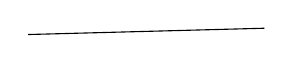
\begin{tikzpicture}\draw (0,0)--(3,0.08);\end{tikzpicture}}

16. Soit $A$ un contracteur non trivial. \unsure{Mes|Les}
\diagram{\begin{tikzcd}
\widehat A \arrow[r,shift left,"i_A"] & Cat \arrow[l,shift left,"j_A"]
\end{tikzcd}}
induisent-ils des équivalences quasi-inverses l'une de l'autre pour les localisés par les \uline{homotopismes} ?

Est-il vrai que $X$ dans $\widehat A$ \unsure{contr.tile|contr.ble} ssi $A_{/X}$ l'est. Que $\forall C$ dans $Cat$ \unsure{contr.tile|contr.ble} si (et seulement si) $A_{/C}\inserted{{}=j_A(C)}$ l'est ? Est-il vrai que pour $X,Y$ dans $\widehat A$, on
\[
i_A(X\times Y)\unsure{\mathbin{-}|\longrightarrow}i_A(X)\times i_A(Y)
\]
un homotopisme ?

\uline{Variantes \unsure{cohomotopes|commutatives}} de ces questions.

\figure{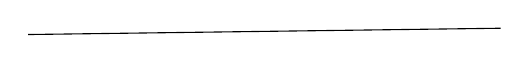
\begin{tikzpicture}\draw (0,0)--(6,0.08);\end{tikzpicture}}

17 Dold-Puppe, Whitehead etc

\figure{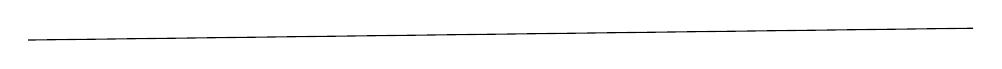
\begin{tikzpicture}\draw (0,0)--(12,.15);\end{tikzpicture}}
\scanpage{6}
% archive foliation: 5
Un topos \unsure{strict} tot. asphérique n'est pas néc. modélisant, même s'il est de la forme $\widehat A$, i.e $A$ n'est pas néc. cat-test. \inserted{et même s'il n'est pas équivalent à $(Ens)$.} Il suffit de prendre une cat $A$ avec \deleted{objet fi-} produits finis, telle que tt objet de $A$ a \uline{une section et une seule}, i.e donc l'objet final est aussi \uline{objet initial},

\deleted{Prendre \unsure{la catégorie|une catégorie} (\unsure{d'anneaux} \illegible{1} \unsure{finis locaux}, \unsure{sur} $k$, à corps résiduel $k$\ldots}

sans pour cela que $A$ soit équiv. à $\Delta_0$.

Mais si $A$ est un contracteur, alors il est cat. test, \uline{sauf} si $A\simeq\Delta_0$.
\cotefile{112}
\scanpage{2}
\uline{Linéarisation}

\margin{\diagram{\begin{array}{r}
\%\\288\\778\\000\\066
\end{array}}}
% archive foliation: 1
% Faint reversed show-through belongs to the opposite face, not to this face.
\scanpage{3}
% archive foliation: 2
\figure{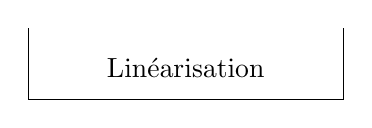
\begin{tikzpicture}\node at (2,0.4) {Linéarisation};\draw (0,.9)--(0,0)--(4,0)--(4,.9);\end{tikzpicture}}

$L\in\mathrm{Ob}\widehat A_{ab}$

On dit que $L$ est lisse si $\forall a\longrightarrow b$ dans $A$,
\diagram{\begin{tikzcd}[row sep=small]
\displaystyle\int_{A_a}L_a \arrow[r] \arrow[d,phantom,"\wr"] & \displaystyle\int_{A_b}L_b \arrow[d,phantom,"\wr"] \\
\displaystyle\int_A L^{(a)} \arrow[d,phantom,"\wr"] & \displaystyle\int_A L^{(b)} \arrow[d,phantom,"\wr"] \\
L^{(a)}*L_\bullet^{A^\circ} & L^{(b)}*L_\bullet^{A^\circ}
\end{tikzcd}}
est un quasi-iso.

On dit que $L$ est \uline{négligeable} si $L^{\unsure{b|\flat}}$ est quasi $=0$ (``quasi-nul'')

i.e. si $\displaystyle\int_{A_a}L=\int_A L^{(a)}$ est \uline{quasi-nul} pour tt $a$ de $A$.

\margin{Soit donc $L^{\unsure{b|\flat}}=(a\longmapsto L^{(a)}*L_\bullet^{A^\circ})$ dans $D_\bullet(\widehat B_{ab})$ c'est un complexe de chaînes dans $\widehat B_{ab}$ qui est \unsure{coh.}$^{\unsure{t}}$ loc.$^t$ constant, i.e. un ``\uline{syst. de coeff tordus}''.}

\margin{\unsure{p-iso} $L\longrightarrow L'$}

Soit \deleted{$\unsure{W}\,\unsure{\widehat A}$} $Lisse_{\mathbb Z}(A)$ la sous-cat pleine de $\widehat A_{ab}$ formée des objets lisses,

\margin{Lisse}

\textcircled{1} $\deleted{Lisse}\,W_{\unsure{q}}^{-1}Lisse_{\mathbb Z}(A)\longrightarrow D_\bullet^{l.c.}(\widehat B_{ab})$ \uline{est-ce une équivalence de catégories} ?

\diagram{\begin{tikzcd}[row sep=small]
D_\bullet^{l.c.}(\widehat B_{ab}) \arrow[d,phantom,"\unsure{\wr|?}"] \\
D_\bullet^{l.c.}(\widehat A_{ab}) \arrow[d,phantom,"\wr"] \\
\left[D_\bullet(Ab)\simeq Hot_{ab}\quad\text{si }A\text{ est asphérique}\right]
\end{tikzcd}}
\margin{par Quillen, peut se définir aussi comme $M_\bullet\longmapsto M_\bullet^{\unsure{b|\flat}}$}

\margin{OK pour $A=\Delta$, mais est-ce OK pour $A=\Delta_{/X}$, où $X\in\mathrm{Ob}\widehat\Delta$ ?}
\margin{$M_\bullet$}

\margin{\uline{NB} Si $A$ est tot. asph., \unsure{alors} \unsure{tous} les \unsure{pt} de $\widehat A_{ab}$ \unsure{quasi iso}}

\textcircled{2} Si $L,M$ dans $Lisse_{\mathbb Z}(A)$, a-t-on
\[
\mathrm{Ext}_{\mathbb Z_A}^i(L,M)\longrightarrow
\mathrm{Ext}_{\mathbb Z_B}^i(L^{\unsure{b|\flat}},M^{\unsure{b|\flat}})
\qquad\text{pour }i>0
\]
\margin{$\left[\simeq\mathrm{Ext}_{\mathbb Z}^i\left(\int_A L,\int_A M\right)\text{ si }A\text{ asph}\right.$}

[serait-ce vrai même sans supposer $L,M$ lisses ? \inserted{et peut-on y remplacer $L,M$ par $L_\bullet,M_\bullet$ ?}]

\textcircled{3} Supposons $L$ lisse, \deleted{et $H_i(L^{\unsure{b|\flat}})=0$ pour $i<N$. On cherche un $L'$,}
\inserted{et $N\in\mathbb N$. On cherche $L'\in\mathrm{Ob}\widehat A_{ab}$ et}
$L\longrightarrow L'$, tel que $L^{\unsure{b|\flat}}\longrightarrow L'^{\unsure{b|\flat}}$ identifie $L'^{\unsure{b|\flat}}$ au tronqué \inserted{homotopiq.} de $L^{\unsure{b|\flat}}$ en degrés $\unsure{\le|<}N$
\scanpage{4}
% archive foliation: 3
\[
L_\bullet\longmapsto\varphi(L_\bullet)
\]
\[
H_i(L_\bullet)\simeq H_i\varphi(L_\bullet)
\]

A) $D_{lc}^b(\widehat A_k)$ etc

B) \diagram{\begin{tikzcd}
D_{lc}^-(\widehat A_k) \arrow[r,shift left] & D_{lc}^-(\widehat B_k) \arrow[l,shift left]
\end{tikzcd}}
\uline{équiv. cat.} \unsure{quasi-inv.} l'une de l'autre

\uline{NB} On a $\unsure{=}$ $D^-(\widehat A_k)\longrightarrow D^-(\widehat B_k)$

C) Objets \uline{lisses} de $\widehat A_k$ (plus gén, de $D^-(\widehat A_k)$, mais c'est moins intéressant)

$\deleted{Lisse_k}\quad \widehat A_{k\text{-lisse}}\qquad \mathbf W\qquad W_{lisse}^{-1}$

\margin{4.11.}

\diagram{\begin{array}{|l|}\hline
c\text{-lisse}\\ c\text{-propre}\\\hline
\end{array}}

\diagram{\begin{tikzcd}[row sep=small,column sep=small]
& & \deleted{A} \\
& X \arrow[d,Rightarrow] & X_{/b}\arrow[d,dash] \\
\mathbb Z^{(X/Y)}\arrow[r] & Y\arrow[r,equal] & Y_{/b} \\
& & \deleted{\unsure{B}}
\end{tikzcd}}

$\deleted{\mathbb Z^{(X)}\unsure{\times Y|_{\times Y}}\simeq\mathbb Z},$

$\widehat A_k$

${}_b\backslash Y$

\uline{lisse}\qquad \uline{colisse}

$\widehat A_M$

$\unsure{\mathbb L}H_\bullet(L\mid A_{/a})$

$\deleted{\unsure{RH}}$

$\unsure{\mathbb L}H^\bullet(L^\circ({}_b B))$

\diagram{\begin{tikzcd}[column sep=small,row sep=small]
{}_b\backslash Y\arrow[r] & Y \\
& {}_{b'}\backslash Y\arrow[ul]\arrow[u]
\end{tikzcd}}

\diagram{\begin{tikzcd}[column sep=small,row sep=small]
{} & {}\arrow[l] \\
b\arrow[dr] & \\
& b'
\end{tikzcd}}
% The pale blue printer characters are reversed show-through, not text on this face.
\scanpage{5}
% archive foliation: 4
\diagram{\begin{array}{llll}
\texttt{09:40:12} & \texttt{0.0242} & \texttt{CSP} & \texttt{JOBNAME GUTS1   SQ 55958} \\
\texttt{09:40:12} & \texttt{0.0242} & \texttt{CSP} & \texttt{TIME EXECUTING IN CPU - 00:00:00.0242} \\
\texttt{09:40:12} & \texttt{0.0242} & \texttt{CSP} & \texttt{TIME WAITING TO EXECUTE 00:00:07.6248} \\
\texttt{09:40:12} & \texttt{0.0242} & \texttt{CSP} & \texttt{TIME WAITING FOR I/O -- 00:00:01.2005} \\
\texttt{09:40:12} & \texttt{0.0243} & \texttt{CSP} & \texttt{MEMORY USAGE ---     0.04790 MWDS-SEC} \\
\texttt{09:40:12} & \texttt{0.0243} & \texttt{CSP} & \texttt{DISK BLOCKS MOVED -----      265} \\
\texttt{09:40:12} & \texttt{0.0243} & \texttt{CSP} & \texttt{PHYSICAL I/O REQUESTS -       29} \\
\texttt{09:40:12} & \texttt{0.0243} & \texttt{CSP} & \texttt{} \\
\texttt{09:40:12} & \texttt{0.0243} & \texttt{CSP} & \texttt{} \\
\texttt{09:40:12} & \texttt{0.0243} & \texttt{CSP} & \texttt{} \\
\texttt{09:40:12} & \texttt{0.0243} & \texttt{USER} & \texttt{TIME WAITING FOR JXT-             00:02:21.1570} \\
\texttt{09:40:12} & \texttt{0.0243} & \texttt{USER} & \texttt{OPEN CALLS-                               14} \\
\texttt{09:40:12} & \texttt{0.0243} & \texttt{USER} & \texttt{CLOSE CALLS-                              10} \\
\texttt{09:40:12} & \texttt{0.0243} & \texttt{USER} & \texttt{MEMORY RESIDENT DATASETS-                   0} \\
\texttt{09:40:12} & \texttt{0.0243} & \texttt{USER} & \texttt{TEMPORARY FILE SPACE USED-                  2 BLOCKS} \\
\texttt{09:40:12} & \texttt{0.0243} & \texttt{USER} & \texttt{PERMANENT FILE SPACE ACCESSED-              0 BLOCKS} \\
\texttt{09:40:12} & \texttt{0.0243} & \texttt{USER} & \texttt{PERMANENT FILE SPACE SAVED-                 0 BLOCKS} \\
\texttt{09:40:12} & \texttt{0.0243} & \texttt{USER} & \texttt{MINIMUM MEMORY USED-                   28160 WORDS} \\
\texttt{09:40:12} & \texttt{0.0243} & \texttt{USER} & \texttt{MAXIMUM MEMORY USED-                   44032 WORDS} \\
\texttt{09:40:12} & \texttt{0.0244} & \texttt{USER} & \texttt{MEMORY INTEGRAL (EXECUTION TIME)-     0.00105 MWDS-SEC} \\
\texttt{09:40:12} & \texttt{0.0244} & \texttt{USER} & \texttt{MEMORY INTEGRAL (I/O WAIT TIME)-      0.04686 MWDS-SEC} \\
\texttt{09:40:12} & \texttt{0.0244} & \texttt{USER} & \texttt{BLOCKS RECEIVED FROM FRONT END-             0} \\
\texttt{09:40:12} & \texttt{0.0244} & \texttt{USER} & \texttt{BLOCKS SENT TO THE FRONT END-               1} \\
\texttt{09:40:12} & \texttt{0.0244} & \texttt{USER} & \texttt{} \\
\texttt{09:40:12} & \texttt{0.0244} & \texttt{USER} & \texttt{} \\
\texttt{09:40:12} & \texttt{0.0244} & \texttt{USER} & \texttt{} \\
\texttt{09:40:12} & \texttt{0.0244} & \texttt{USER} & \unsure{\texttt{********************************************************************************}} \\
\texttt{09:40:12} & \texttt{0.0244} & \texttt{USER} & \texttt{*                                                                              *} \\
\texttt{09:40:12} & \texttt{0.0246} & \texttt{USER} & \texttt{*   CPU TIME USED              0.024 SECONDS         0.03 UC CNRS               *} \\
\texttt{09:40:13} & \texttt{0.0247} & \texttt{USER} & \texttt{*   DISK IO BLOCKS MOVED        0.267 KIOB            0.13 UC CNRS               *} \\
\texttt{09:40:13} & \texttt{0.0248} & \texttt{USER} & \texttt{*   MEMORY USAGE               0.001 MWDS-SCPU       0.00 UC CNRS               *} \\
\texttt{09:40:13} & \texttt{0.0250} & \texttt{USER} & \texttt{*                              0.047 MWDS-SIOW       0.02 UC CNRS               *} \\
\texttt{09:40:13} & \texttt{0.0250} & \texttt{USER} & \texttt{*                                                                              *} \\
\texttt{09:40:13} & \texttt{0.0251} & \texttt{USER} & \texttt{*   TOTAL SBUS USED                                  1.19 UC CNRS               *} \\
\texttt{09:40:13} & \texttt{0.0251} & \texttt{USER} & \texttt{*                                                                              *} \\
\texttt{09:40:13} & \texttt{0.0251} & \texttt{USER} & \unsure{\texttt{********************************************************************************}} \\
\end{array}}

% Handwriting to the right of the printed listing, from its top down.
\[
F*k^{(b_\beta^\circ)}\simeq F(b_\beta)
\]
\[
\underbrace{L^{(a)}*k^{(b_\beta^\circ)}}_{G(a)\ \text{où }a\in A}
\simeq L(b_\beta)^{(\mathrm{Hom}_A(b_\beta,a))}
\]
\[
\begin{aligned}
x&\longmapsto\left[k^{(a_\alpha)}*G^{(x^\circ)}
 \simeq G_{\unsure{i}\deleted{\unsure{a}}}^{(x^\circ)}(a_\alpha^\circ)\right.\\
&\simeq G(a_\alpha)^{(\mathrm{Hom}_{\unsure{B}}(a_\alpha^\circ,x^\circ))}\\
&\simeq G(a_\alpha)^{(\mathrm{Hom}_A(x,a_\alpha))}\\
&\simeq L(b_\beta)^{(\mathrm{Hom}_A(b_\beta,a_\alpha)\times\mathrm{Hom}_A(x,a_\alpha))}
\end{aligned}
\]
\[
x\longmapsto\bigoplus_{\alpha,\beta,i}L_i(b_\beta)^{(\mathrm{Hom}(b_\beta,a_\alpha)\times\mathrm{Hom}_A(x,a_\alpha))}
\]
\margin{$L_i^{(\mathrm{Hom}(X,a_\alpha))}$}

$D^b$

\figure{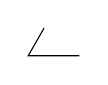
\begin{tikzpicture}\draw (.2,.35)--(0,0)--(.65,0);\end{tikzpicture}}
\diagram{\left\{\begin{tikzcd}[row sep=small]
\unsure{LH}_\bullet^{(k)}\ \text{\unsure{appl. diag.}} & {} \\
DR_k\ \text{\unsure{opérat. dér.}} & \\
Add_k(A)\arrow[uur,bend right]\arrow[d,Rightarrow] & {}\arrow[uu]\arrow[ul,Rightarrow] \\
D_{lc}^b(\widehat A_k) &
\end{tikzcd}\right.}

\[
D_{lc}^b(\widehat A_k)\longrightarrow D_{lc}^b(\widehat{\unsure{B}}_k)
\]
\[
L_\bullet\qquad a\longmapsto\underbrace{L_\bullet^{(a)}*L_\bullet^B}
\qquad M=\coprod_{\unsure{J}}
\]
\[
\bigoplus_{i,\alpha,\beta}
\left(L_i(b_\beta)^{(\mathrm{Hom}(b_\beta,a_\alpha))}*k^{(a_\alpha)}\right)
\]
\margin{$L_i(b_\beta)^{(a_\alpha)}$}
\[
b\longmapsto M_{i\beta}^{(b)}
\]
\[
\underbrace{k^{(a_\alpha)}*\left[a\longmapsto
\left(L_i^{(a)}*k^{(b_\beta^\circ)}\right)\right]}_{M_{i\beta}}
=\int L_i(b_\beta)^{\mathrm{Hom}(b_\beta,a)}
\]
\margin{$M_{i\beta}^{(b)}$}
\[
k^{(a_\alpha)}*\left[b\longmapsto M_{i\beta}^{(b)}\right]
\simeq M_{i\beta}(a_\alpha)^{(\mathrm{Hom}_A(b,a_\alpha))}
\]
\[
b\longmapsto \deleted{\unsure{L}}\bigoplus_{\alpha,\beta}
L_i(b_\beta)^{(\mathrm{Hom}(b_\beta,a_\alpha)\times\mathrm{Hom}(b,a_\alpha))}
\]
\cotefile{113}
\scanpage{2}
% archive number at upper left: 377
Abelianization

\texttt{0MIN 00.02SEC VIRT 84K SYS 256K}

\texttt{0MIN 00.02SEC}

\margin{\unsure{9.}}
% archive foliation: 1
\scanpage{3}
% archive foliation: 2
\diagram{\begin{tikzcd}
\alpha\arrow[r,Rightarrow]\arrow[d,"\unsure{\zeta|\xi}"']&\beta\arrow[d,dashed]&\gamma\arrow[l,hook']\arrow[d,"\eta"]\\
X\arrow[r,Rightarrow]&Y&Z\arrow[l,hook']
\end{tikzcd}}

\diagram{\begin{tikzcd}[column sep=tiny,row sep=large]
\alpha_0\arrow[r,Rightarrow]\arrow[d,"\unsure{\zeta|\xi}_0"'] & \alpha'_0\deleted{\unsure{\alpha_1}}\arrow[d,dotted,"\unsure{\zeta|\xi}'_0"]\arrow[dr,"\eta_0"]\arrow[rrrrrr,bend left,"u",dash] & \alpha_1\arrow[l,hook']\arrow[r]\arrow[d,"\unsure{\zeta|\xi}_1"]\arrow[dr,"\eta_1"] & \alpha_2\arrow[r]\arrow[d,"\unsure{\zeta|\xi}_2"]\arrow[dr,"\eta_2"] & \alpha_{n-2}\arrow[r]\arrow[d,"\unsure{\zeta|\xi}_{n-2}"]\arrow[dr,"\unsure{\eta_{n-2}}"] & \alpha_{n-1}\arrow[r,Rightarrow]\arrow[d,"\unsure{\zeta|\xi}_{n-1}"]\arrow[dr,"\eta_{n-1}"] & \alpha'_{n-1}\arrow[d,dotted,"\unsure{\zeta|\xi}'_{n-1}"] & \alpha_n\arrow[l,hook']\arrow[d,"\unsure{\zeta|\xi}_n"]\\
X_0\arrow[r,Rightarrow]&X'_0\arrow[rrrrrr,bend right,"v"',dash]&X_1\arrow[l,hook']\arrow[r]&X_2\arrow[r,dash,"\cdots"]&X_{n-2}\arrow[r,dash]&X_{n-1}\arrow[r,Rightarrow]&X'_{n-1}&X_n\arrow[l,hook']
\end{tikzcd}}

Les syst. $(\unsure{\zeta|\xi}'_0,\unsure{\zeta|\xi}'_{n-1})$ tels que $\unsure{\zeta|\xi}'_{n-1}u=v\unsure{\zeta|\xi}'_0$ forment \deleted{\unsure{un} multibimodule} $MU$-fibré $M_1$

$M\longrightarrow$ foncteur des syst. $\eta_{\unsure{0|i}}$

\deleted{\diagram{\begin{tikzcd}M\arrow[r,"\mathrm{subm}"']&M_1\end{tikzcd}}}

\diagram{\begin{tikzcd}[column sep=small,row sep=small]
M(\unsure{\zeta|\xi}_0,\unsure{\zeta|\xi}_n)\arrow[r,"\mathrm{subm}"']&M(\unsure{\zeta|\xi}'_0,\unsure{\zeta|\xi}'_n)\arrow[d]\\
M(\unsure{\zeta|\xi}'_0,\eta_0,\ldots,\eta_{n-1},\unsure{\zeta|\xi}'_n)\arrow[ur,dash]&M(\eta_0,\eta_{n-1})\\
&M(\eta_0,\eta_1,\ldots,\eta_{n-1})\arrow[u,"\mathrm{subm}"']
\end{tikzcd}}

\deleted{\diagram{\begin{tikzcd}[row sep=small]
M(\unsure{\zeta|\xi}_0,\unsure{\zeta|\xi}'_0)\times M(\unsure{\zeta|\xi}'_n,\unsure{\zeta|\xi}_n)\arrow[d]\\
M(\unsure{\unsure{\zeta|\xi}'_0,\eta_0})\times M(\unsure{\eta_{n-1},\unsure{\zeta|\xi}'_n})\arrow[d]\\
M(\unsure{\zeta|\xi}'_0,\unsure{\zeta|\xi}'_n)
\end{tikzcd}}}

\diagram{\begin{tikzcd}[column sep=small,row sep=large]
& M(\unsure{\zeta|\xi}_0,\unsure{\zeta|\xi}'_0,\unsure{\zeta|\xi}_1,\ldots,\unsure{\zeta|\xi}_{n-1},\unsure{\zeta|\xi}'_{n-1},\unsure{\zeta|\xi}_n)=M(\eta_0,\eta_1,\ldots,\eta_{n-1})\arrow[d,"\uline{\mathrm{subm}}"] & \\
\deleted{M(\unsure{\zeta|\xi}_0,\unsure{\zeta|\xi}_n)}\arrow[d] & M(\unsure{\zeta|\xi}'_0,\unsure{\zeta|\xi}_1,\unsure{\zeta|\xi}_2,\ldots,\unsure{\zeta|\xi}_{n-1},\unsure{\zeta|\xi}'_n)\arrow[d,"\uline{\mathrm{subm}}"]\arrow[r]\arrow[dr,phantom,"\mathrm{cart}"]&\displaystyle\prod_{0\le i\le n-2}M(\eta_i,\unsure{\zeta|\xi}_{i+1},\eta_{i+1})\arrow[d,"{\text{\tikz[baseline=(s.base)]{\node[draw,ellipse,inner sep=1pt](s){subm};}}}"]\\
M(\unsure{\zeta|\xi}'_0,\unsure{\zeta|\xi}'_n)\arrow[d]\arrow[r,phantom,"\mathrm{cart}"] & M(\unsure{\zeta|\xi}'_0,\eta_0,\eta_1,\ldots,\eta_{n-1},\unsure{\zeta|\xi}'_n)\arrow[l,"\uline{\mathrm{subm}}"']\arrow[d]\arrow[r]&\displaystyle\prod_{0\le i\le n-2}M(\eta_i,\eta_{i+1})\\
M(\eta_0,\eta_{n-1})&M(\eta_0,\eta_1,\ldots,\eta_{n-1})\arrow[l,"{\text{\tikz[baseline=(s.base)]{\node[draw,ellipse,inner sep=1pt](s){subm};}}}\ (\uline{\mathrm{r\acute ecur}})"']&
\end{tikzcd}}

\diagram{\begin{tikzcd}[column sep=small,row sep=small]
M(\unsure{\zeta|\xi}'_0,1)\times M(1,\unsure{\zeta|\xi}'_n)\arrow[d,"\mathrm{subm}"'] &\deleted{\unsure{M(\unsure{\zeta|\xi}_0,\unsure{\zeta|\xi}_n)}}\arrow[l]\arrow[d]&\inserted{M(\unsure{\zeta|\xi}'_0,\unsure{\zeta|\xi}'_n)}\arrow[d,"\mathrm{subm}"]\\
M(\eta_0,1)\times M(1,\eta_{n-1})& {} &M(\unsure{\zeta|\xi}'_0,\unsure{\zeta|\xi}'_n)\arrow[ll,"\mathrm{cart}"']\arrow[dl,"\uline{\mathrm{subm}}"]\\
&e&
\end{tikzcd}}
\margin{\deleted{\unsure{subm}}}
\margin{\figure{\begin{tikzpicture}\draw[->] (1.5,1)--(0,0);\draw[dashed,->] (1.2,.1)--(.3,-.5);\end{tikzpicture}}}

\deleted{Pour que $\displaystyle\int_I X(i)$ ne fasse pas sortir des $MU$-fibrés semi-simpliciaux, il suffit que}

\deleted{a) $\mathrm{Nerf}(I)$ asphérique i.e. $I$ asphérique}

\deleted{b) Chaque $X(i)$ transforme op. bord $d_i:\Delta_{n-1}\longrightarrow\Delta_n$ en submersions}

\deleted{c) $\forall u\in\mathrm{Fl}(I)$, $u:i\longrightarrow j$, $X(u):X(i)\longrightarrow X(j)$ se factorise en $gf$, avec $f$ subm, $g$ mono.}

\margin{\diagram{\begin{tikzcd}[column sep=small,row sep=small]
\alpha\arrow[r,Rightarrow]\arrow[d,"\unsure{\zeta|\xi}_0"']&\deleted{\unsure{\beta}}\arrow[d,"\deleted{\unsure{\unsure{\zeta|\xi}'}}"]&\unsure{\beta}\arrow[l,dash]\arrow[d,"\unsure{\zeta|\xi}_1"]\\
X\arrow[r,Rightarrow]&Y&Z\arrow[l,hook']
\end{tikzcd}}}
\scanpage{4}
\mspage{\textcircled{1}}
\margin{\fbox{$\unsure{\otimes}$ dans $Cat$}}
$P$ petite catégorie $k$-additive
\[
P^{\unsure{\&}}\deleted{{}^{\unsure{*}}}\mathrel{\mathop=^{\rm def}}
\underline{\mathrm{Hom}}_{\mathbf Z}(P^\circ,Ab)\simeq
\underline{\mathrm{Hom}}_k(P^\circ,Ab_k)
\]
\margin{(ne dépend pas du choix de la str. $k$-additive)}
$P\hookrightarrow P^{\unsure{\&}}$ inclusion additive pl. fid. d'où
\[
\operatorname{Kar}P\longrightarrow P^{\unsure{\&}}
\quad\text{qui induit équivalence}\qquad
\operatorname{Kar}P\xrightarrow{\simeq}\operatorname{UlProj}(P^{\unsure{\&}})
\]
\margin{\uline{NB} $P\longrightarrow\operatorname{Kar}P$ induit
$(\operatorname{Kar}P)^{\unsure{\&}}\xrightarrow{\simeq}P^{\unsure{\&}}$.}
Soit $\mathcal P$ catégorie, \inserted{$k$-additive}, pour qu'elle soit
\inserted{$\simeq$ cat} de la forme $P^{\unsure{\&}}$, avec $P$ additive,
il f. et s. que
\[
\left\{\begin{array}{ll}
\text{a)}&\mathcal P\text{ est un \uline{topos abélien} i.e. cat \uline{abélienne},}\\
&\text{stable par petites }\varinjlim\text{ filtrantes celles-ci}\\
&\text{étant exactes, et admettant une petite}\\
&\text{sous-cat. génératrice}\\
\text{b)}&\mathcal P\text{ a assez de projectifs.}
\end{array}\right.
\]
\deleted{\unsure{Pour cela}} \inserted{et alors}
On a une \inserted{$k$-}équivalence $\mathcal P\simeq P^{\unsure{\&}}$,
avec $P$ $k$-add.
(et on peut prendre $P=\operatorname{UlProj}(\mathcal P)$).
\diagram{\begin{tikzcd}
(Add_k) \arrow[r,"\text{2-ess. surj}","\deleted{\unsure{2-fid}}"']
\arrow[d,"\operatorname{Kar}"'] & (Top\,ab\,\unsure{alg}_k)\\
(AddKar_k)\arrow[ur,"\unsure{3-fid.}"] &
\end{tikzcd}}
morphismes de topos $k$-abéliens \unsure{alg}
sont les $f_!:\mathcal P\longrightarrow\mathcal Q$ commutant aux $\varinjlim$
telles que $f^*$ \deleted{\unsure{commute}} (son adjoint à droite) commute
aux $\varinjlim$, i.e. admet adjoint à droite $f_*$.

Soit $L\in\operatorname{Ob}P^{\unsure{\&}}$, alors
\[
L\longleftarrow\varinjlim_{P/L}a
\]
\diagram{\begin{tikzcd}[column sep=large]
\underline{\mathrm{Hom}}_{k!}(P^{\unsure{\&}},\deleted{Ab_k}\inserted{M})
\arrow[r,"\simeq"]\arrow[d,"\deleted{\simeq}"'] &
\underline{\mathrm{Hom}}_k(P,\deleted{Ab_k}\inserted{M})
\arrow[d,"\deleted{\simeq}"]\\
\deleted{\underline{\mathrm{Hom}}_{\mathbf Z!}(P^{\unsure{\&}},Ab)}
\arrow[r,"\deleted{\simeq}"] &
\deleted{\underline{\mathrm{Hom}}_{\mathbf Z\unsure{!}}(P,Ab)}
\end{tikzcd}}
\margin{si $M$ $k$-additive st.\unsure{ble} par $\varinjlim$}
\[
\underline{\mathrm{Hom}}_k^!(P^{\unsure{\&}\circ},M)
\xrightarrow{\simeq}\underline{\mathrm{Hom}}_k(P^\circ,M)
\qquad\text{si }M\text{ $k$-additive st.\unsure{ble} par }\varprojlim.
\]
Soit $Q=P^\circ$
\[
\underline{\mathrm{Hom}}_k^!(Q^{\unsure{\&}\circ},M)
\xrightarrow{\simeq}\underline{\mathrm{Hom}}_k(P,M)
\]
% archive foliation: 3
\scanpage{5}
\margin{\texttt{//*\ \ GUTS\ \ \unsure{STC0}\ \ \unsure{1}}}
\diagram{\begin{array}{l}
\texttt{\ GGGGGGGGGG\ \ \ UU\ \ \ \ \ \ \ \ UU\ \ TTTTTTTTTTTT\ \ \ SSSSSSSSSS\ } \\
\texttt{GGGGGGGGGGGG\ \ UU\ \ \ \ \ \ \ \ UU\ \ TTTTTTTTTTTT\ \ SSSSSSSSSSSS} \\
\texttt{GG\ \ \ \ \ \ \ \ GG\ \ UU\ \ \ \ \ \ \ \ UU\ \ \ \ \ \ \ TT\ \ \ \ \ \ \ SS\ \ \ \ \ \ \ \ SS} \\
\texttt{GG\ \ \ \ \ \ \ \ \ \ \ \ UU\ \ \ \ \ \ \ \ UU\ \ \ \ \ \ \ TT\ \ \ \ \ \ \ SS} \\
\texttt{GG\ \ \ \ \ \ \ \ \ \ \ \ UU\ \ \ \ \ \ \ \ UU\ \ \ \ \ \ \ TT\ \ \ \ \ \ \ SSS} \\
\texttt{GG\ \ \ \ \ \ \ \ \ \ \ \ UU\ \ \ \ \ \ \ \ UU\ \ \ \ \ \ \ TT\ \ \ \ \ \ \ \ SSSSSSSSS} \\
\texttt{GG\ \ \ \ \ GGGGG\ \ UU\ \ \ \ \ \ \ \ UU\ \ \ \ \ \ \ TT\ \ \ \ \ \ \ \ \ SSSSSSSSS} \\
\texttt{GG\ \ \ \ \ GGGGG\ \ UU\ \ \ \ \ \ \ \ UU\ \ \ \ \ \ \ TT\ \ \ \ \ \ \ \ \ \ \ \ \ \ \ \ SSS} \\
\texttt{GG\ \ \ \ \ \ \ \ GG\ \ UU\ \ \ \ \ \ \ \ UU\ \ \ \ \ \ \ TT\ \ \ \ \ \ \ \ \ \ \ \ \ \ \ \ \ SS} \\
\texttt{GG\ \ \ \ \ \ \ \ GG\ \ UU\ \ \ \ \ \ \ \ UU\ \ \ \ \ \ \ TT\ \ \ \ \ \ \ SS\ \ \ \ \ \ \ \ SS} \\
\texttt{GGGGGGGGGGGG\ \ UUUUUUUUUUUU\ \ \ \ \ \ \ TT\ \ \ \ \ \ \ SSSSSSSSSSSS} \\
\texttt{\ GGGGGGGGGG\ \ \ \ UUUUUUUUUU\ \ \ \ \ \ \ \ TT\ \ \ \ \ \ \ \ SSSSSSSSSS}
\end{array}}
\diagram{\begin{array}{llllllllllllllll}
\texttt{****P}&\texttt{END}&\texttt{STC}&180&\texttt{GUTS}&\texttt{ROOM}&11.07.13&\texttt{AM}&16&\texttt{SEP}&82&\texttt{R6.PR1}&\texttt{SYS JES2}&\texttt{STC 180}&\texttt{END}&\texttt{P****} \\
\texttt{****P}&\texttt{END}&\texttt{STC}&180&\texttt{GUTS}&\texttt{ROOM}&11.07.13&\texttt{AM}&16&\texttt{SEP}&82&\texttt{R6.PR1}&\texttt{SYS JES2}&\texttt{STC 180}&\texttt{END}&\texttt{P****} \\
\texttt{****P}&\texttt{END}&\texttt{STC}&180&\texttt{GUTS}&\texttt{ROOM}&11.07.13&\texttt{AM}&16&\texttt{SEP}&82&\texttt{R6.PR1}&\texttt{SYS JES2}&\texttt{STC 180}&\texttt{END}&\texttt{P****} \\
\texttt{****P}&\texttt{END}&\texttt{STC}&180&\texttt{GUTS}&\texttt{ROOM}&11.07.13&\texttt{AM}&16&\texttt{SEP}&82&\texttt{R6.PR1}&\texttt{SYS JES2}&\texttt{STC 180}&\texttt{END}&\texttt{P****} \\
\texttt{****P}&\texttt{END}&\texttt{STC}&180&\texttt{GUTS}&\texttt{ROOM}&11.07.13&\texttt{AM}&16&\texttt{SEP}&82&\texttt{R6.PR1}&\texttt{SYS JES2}&\texttt{STC 180}&\texttt{END}&\texttt{P****} \\
\texttt{****P}&\texttt{END}&\texttt{STC}&180&\texttt{GUTS}&\texttt{ROOM}&11.07.13&\texttt{AM}&16&\texttt{SEP}&82&\texttt{R6.PR1}&\texttt{SYS JES2}&\texttt{STC 180}&\texttt{END}&\texttt{P****}
\end{array}}
% archive foliation: 4
\scanpage{6}
\mspage{\textcircled{2}}
\[
\underbrace{\underline{\mathrm{Hom}}_k^!(Q^{\unsure{\&}\circ},M)}_{\mathcal Q_M}
\simeq
\underbrace{\underline{\mathrm{Hom}}_{k!}(P^{\unsure{\&}},M)}_{\mathcal P^M}
\qquad\text{si }M\text{ $k$-add. st.\unsure{ble} par les deux types de lim}
\]
Sur $\mathcal P_M^{\deleted{\unsure{\&}}}\xrightarrow{\simeq}
\underline{\mathrm{Hom}}_k(P^\circ,M)$
\[
\mathcal Q=\mathcal P^\vee\text{ opère par }(F,L')\longmapsto F*_kL'
\]
\margin{$\overbrace{\mathcal P_M^{\deleted{\unsure{\&}}}\times\mathcal Q}^{P_M^{\unsure{\&}}\times Q^{\unsure{\&}}}\longrightarrow M$}
\[
\mathcal P\text{ opère par }(L,F)\longmapsto\underline{\mathrm{Hom}}_k(L,F)
\]
\margin{$\underbrace{\mathcal P\times\mathcal P_M^{\unsure{!}}}_{P^{\unsure{\&}}\times P_M^{\unsure{\&}}}\longrightarrow M$}
On a
\[
(\underbrace{F*_kL'}_{P,M})^\circ\simeq\deleted{\unsure{E}}
\underbrace{\underline{\mathrm{Hom}}_k(L',F^\circ)}_{Q,M^\circ}
\]
\[
(\overbrace{\underline{\mathrm{Hom}}_k(L,F)}^{P,M})^\circ
\simeq\overbrace{F^\circ*L}^{Q,M^\circ}
\qquad\deleted{\unsure{\underbrace{\phantom{Hom}}}}
\]
\deleted{$\unsure{\mathcal Q^\circ\simeq\mathcal P}$}
\figure{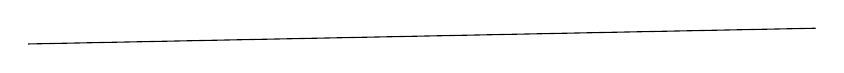
\begin{tikzpicture}\draw (0,0)--(10,.2);\end{tikzpicture}}

Soient $P,Q$ $k$-additives, on définit $P\otimes_kQ$ et
$\underbrace{P\times Q\unsure{-|\longrightarrow}P\otimes_kQ}_{k\text{-biadditive}}$
de façon 2-universelle :
\[
\underline{\mathrm{Hom}}_k(P\otimes_kQ,M)\simeq\operatorname{Bil}_k(P,Q;M)
\qquad\text{tout }M\text{ $k$-additive}
\]
Construction explicite par familles finies d'objets de $P\times Q$
\[
\unsure{\zeta|\xi}=\bigoplus_{i\in I}a_i\otimes_k b_i
\]
avec, pour
\[
\unsure{\zeta|\xi}'=\bigoplus_{j\in\unsure{J|I}}a'_j\otimes_k b'_j
\]
\[
\mathrm{Hom}(\unsure{\zeta|\xi},\unsure{\zeta|\xi}')=
\prod_{I\times J}\mathrm{Hom}(a_i,a'_j)\otimes_k\mathrm{Hom}(b_i,\unsure{b'_j|b_j})
\]
À retenir

 a) Si $P,Q$ petites, $P\otimes_kQ$ est petite
\[
\text{b)}\quad
\mathrm{Hom}_{P\otimes_kQ}(a\otimes_kb,a'\otimes_kb')
\xleftarrow{\sim}\mathrm{Hom}_P(a,a')\otimes_k\mathrm{Hom}_Q(b,b')
\]
On en conclut que le foncteur \inserted{can} (pl. fid !)
% archive foliation: 5
\scanpage{7}
\diagram{\begin{array}{l}
\texttt{END} \\
\texttt{//LKED.SYSLIB\ DD} \\
\texttt{//\ \ \ \ \ \ \ \ \ DD\ \ DSN=CNU1.MODULEF.UTIM,DISP=SHR} \\
\texttt{//\ \ \ \ \ \ \ \ \ DD\ \ DSN=CNU1.MODULEF.\unsure{UTDL|UTOL},DISP=SHR} \\
\texttt{//\ \ \ \ \ \ \ \ \ DD\ \ DSN=CNU1.MODULEF.UTIF,DISP=SHR} \\
\texttt{//\ \ \ \ \ \ \ \ \ DD\ \ DSN=CNU1.MODULEF.UTIL,DISP=SHR} \\
\texttt{//\ \ \ \ \ \ \ \ \ DD\ \ DSN=CNU1.MODULEF.UTSD,DISP=SHR} \\
\texttt{//\ \ \ \ \ \ \ \ \ DD\ \ DSN=CNU1.MODULEF.MEFI,DISP=SHR} \\
\texttt{//\ \ \ \ \ \ \ \ \ DD\ \ DSN=CNU1.MODULEF.COSD,DISP=SHR} \\
\texttt{//\ \ \ \ \ \ \ \ \ DD\ \ DSN=CNU1.MODULEF.ELAS,DISP=SHR} \\
\texttt{//GO.FT10F001\ DD\ \ DSN=MAC0446.JCLAPAC.MEFI,DISP=OLD} \\
\texttt{//GO.FT11F001\ DD\ \ DSN=MAC0446.JCLAPAC.NOPO,DISP=OLD} \\
\texttt{//GO.FT12F001\ DD\ \ DSN=MAC0446.JCLAPAC.MAIL,DISP=OLD} \\
\texttt{//GO.FT13F001\ DD\ \ DSN=MAC0446.JCLAPAC.COOR,DISP=OLD} \\
\texttt{//GO.SYSIN\ \ \ DD\ \ *} \\
\texttt{'GENERALITES'} \\
\texttt{'TEST\ D''UNE\ PLAQUE\ 40X40\ DE\ 75\ NOEUDS\ ET\ 116\ ELEMENTS'} \\
\texttt{'29\ 06\ 82'\ 'PATRICK\ CHABRAND'} \\
\texttt{\$NCI,NFC,NDI,NF,NCCF,\unsure{NDSDZ}\$\ 0\ 0\ 0\ 6\ 0\ 1} \\
\texttt{'\unsure{RENGMK|RENGMC}:RENUMEROTATION\ GLOBALE'} \\
\texttt{\$IMP,NFMEFE,NFMEFS,NCROIS,NELRE\$\ 0\ 10\ 10\ 1\ 1} \\
\texttt{\$NPFD,...,NOPFD(L),...\$\ 17\ 12\ 15\ 16\ 19\ 20\ 39\ 36\ 35\ 32\ 70\ 71\ 74\ 61\ 60} \\
\texttt{57\ 56\ 53} \\
\texttt{'MESHPL:TRACE\ DES\ ELEMENTS'} \\
\texttt{\$IMP,NFMEFI,IZOOM,KODE,COORDONNEES\$\ 0\ 10\ 1\ 12\ 0.\ 0.\ 40.\ 40.} \\
\texttt{'MESHPL:NUMERO\ DES\ NOEUDS'} \\
\texttt{\$IMP,NFMEFI,IZOOM,ICODE,COORDONNEES\$\ 0\ 10\ 1\ -2\ 0.\ 0.\ 40.\ 40.} \\
\texttt{'MEFNOP:TRANSFORMATION\ DE\ MEFI\ EN\ SD\ NOPO\ DE\ NIVEAU\ ZERO'} \\
\texttt{\$IMPRE,NFMEFI,NFNOPO,NINOPO,NTNOPO,NANOPO\$\ 7\ 10\ 11\ 0\ 0\ '/N01'} \\
\texttt{'FIN'} \\
\texttt{//}
\end{array}}
% archive foliation: 6
\scanpage{8}
\mspage{\textcircled{3}}
\[
P\otimes_kQ\hookrightarrow(P\otimes_kQ)^{\unsure{\&}}
\simeq\underline{\operatorname{Bil}}_k(P^\circ,Q^\circ;(Ab_k))
\]
est donné par
\[
(*)\qquad a\otimes_kb\longmapsto
\big((x,y)\longmapsto\mathrm{Hom}_P(x,a)\otimes_k\mathrm{Hom}_Q(y,b)\big)
\]
ce qui donne une construction \unsure{directe} de
$P\otimes_kQ$ comme la sous-cat. pleine de
$\underline{\operatorname{Bil}}_k(P^\circ,Q^\circ;Ab_k)$
formée des sommes finies des foncteurs de la forme $(*)$
(\uline{ou} la cat. str. pleine correspondante).

\margin{\figure{\begin{tikzpicture}\draw[->] (0,0)--(1,.5);\end{tikzpicture}}}
\uline{Application 1} Soit $M\simeq Q^{\unsure{\&}}$ un topos $k$-abélien \unsure{alg.},
$M^\vee\simeq Q^{\circ\unsure{\&}}$ ``le'' topos $k$-abélien \unsure{alg.} dual
\margin{(de l'existence de $P\otimes_kQ$, \deleted{\unsure{et}} et du fait qu'il est petit si $P,Q$ le sont)}
Considérons $P_M^{\unsure{\&}}$ et $P_{M^\vee}^{\circ\unsure{\&}}$
($\simeq\mathcal P_M$ et $(\mathcal P^\vee)_{M^\vee}$),
ce sont des topos $k$-abéliens \unsure{alg.}, et en dualité.

En effet,
\[
\begin{aligned}
P_M^{\unsure{\&}}&=\underline{\mathrm{Hom}}_k(P^\circ,\underline{\mathrm{Hom}}_k(Q^\circ,Ab_k))\\
&\simeq\underline{\mathrm{Hom}}_k(\underbrace{P^\circ\otimes_kQ^\circ}_{\rotatebox{90}{$\simeq$}},Ab_k)\\
&\simeq\underline{\mathrm{Hom}}_k(\overbrace{(P\otimes_kQ)^\circ},Ab_k)
=(P\otimes_kQ)^{\unsure{\&}}.
\end{aligned}
\]
donc topos $k$-abélien \unsure{alg.}, de $=$
\[
\begin{aligned}
P_{M^\vee}^{\circ\unsure{\&}}&\simeq\underline{\mathrm{Hom}}_k(
\underbrace{(P^\circ\otimes_kQ^\circ)^\circ},Ab_k)\\
&\simeq\underline{\mathrm{Hom}}(P\otimes_kQ,Ab_k)
=(P\otimes_kQ)^{\circ\unsure{\&}}
\end{aligned}
\]
\uline{Appl. 2}
\[
\underline{\operatorname{Bil}}_{k!!}(P^{\unsure{\&}},Q^{\unsure{\&}};M)
\xleftarrow{\simeq}\deleted{\unsure{Bil}}
\underline{\mathrm{Hom}}_{k!}((P\otimes_kQ)^{\unsure{\&}},M)
\quad(\simeq\operatorname{Bil}_k(P,Q;\unsure{M}))
\]
\margin{si $M$ $k$-add. avec $\varinjlim$}
\margin{$\unsure{*}$}
i.e. $(P^{\deleted{\unsure{\&}}}\otimes_kQ)^{\unsure{\&}}$
joue le rôle de prod. tens. des topos $k$-abél. $P^{\unsure{\&}},Q^{\unsure{\&}}$,
parmi les cat. $k$-additives st.\unsure{bles} par $\varinjlim$
% archive foliation: 7
\scanpage{9}
\diagram{\begin{array}{l}
\texttt{/*JOBPARM\ L=5} \\
\texttt{//\ \ \ \ \ \ \ \ EXEC\ FORTXCLG,PARM.LKED=(LIST,LET,IOMAP),COND.GO=(9,LT),} \\
\texttt{//\ \ \ \ \ \ \ \ REGION.GO=500K} \\
\texttt{//FORT.SYSIN\ DD\ \ *} \\
\texttt{C\ \ \ \ \ ETUDE\ D\ UN\ DOMAINE\ BIDIMENSIONNEL\ ELASTIQUE\ CHAUFFE} \\
\texttt{C\ \ \ \ \ \ MAILLAGE\ DU\ DOMAINE:RENUMEROTATION,CONSTRUCTION\ DE\ LA\ SD\ NOPO} \\
\texttt{C\ \ \ \ \ MAIL\ ET\ COOR.} \\
\texttt{C\ \ \ \ \ SONT\ NECESSAIRES\ LES\ FICHIERS:MEFI(10),EXISTANT\ ET\ LES\ TROIS} \\
\texttt{C\ \ \ \ \ FICHIERS\ NOPO(11),MAIL(12),COOR(13)\ A\ CATALOGUER.} \\
\texttt{\ \ \ \ \ \ DOUBLE\ PRECISION\ DM} \\
\texttt{\ \ \ \ \ \ DIMENSION\ M(10000)} \\
\texttt{\ \ \ \ \ \ DIMENSION\ ICODEL(4)} \\
\texttt{\ \ \ \ \ \ EQUIVALENCE\ (M(1),DM)} \\
\texttt{\ \ \ \ \ \ \ COMMON\ /\unsure{TRAVAI|TRAVA1}/\ IM,LM,NOMTAB,NNN,NTAB(1020)} \\
\texttt{\ \ \ \ \ \ \ COMMON\ /TRAVA1/\ NN(29),IMPRE,IMPLEC,INILEC,IFIL} \\
\texttt{\ \ \ \ \ \ \ NOMTAB=0} \\
\texttt{\ \ \ \ \ \ \ IMPRE=0} \\
\texttt{\ \ \ \ \ \ \ IMPLEC=1} \\
\texttt{\ \ \ \ \ \ \ INILEC=0} \\
\texttt{\ \ \ \ \ \ \ LM=10000} \\
\texttt{\ \ \ \ \ \ \ \ NNN=0} \\
\texttt{\ \ \ \ \ \ \ \ IM=1} \\
\texttt{C} \\
\texttt{C} \\
\texttt{C\ \ \ \ \ RENUMEROTATION\ DE\ LA\ STRUCTURE\ NOPO} \\
\texttt{C} \\
\texttt{\ \ \ \ \ \ \ \ \ \ CALL\ APMEFI(M,M,M)} \\
\texttt{\ \ \ \ \ \ \ \ \ \ IMPRE=10} \\
\texttt{\ \ \ \ \ \ NDIM=2} \\
\texttt{\ \ \ \ \ \ NDSD=0} \\
\texttt{\ \ \ \ \ \ NNR=9} \\
\texttt{\ \ \ \ \ \ NBSDC=0} \\
\texttt{\ \ \ \ \ \ NBSC=0} \\
\texttt{\ \ \ \ \ \ NOSC=0} \\
\texttt{\ \ \ \ \ \ NBLC=0} \\
\texttt{\ \ \ \ \ \ NOLC=0} \\
\texttt{C} \\
\texttt{\ \ \ \ \ \ NOPOEX=1} \\
\texttt{\ \ \ \ \ \ IDTECA=0} \\
\texttt{\ \ \ \ \ \ NOMBIB=NOMAFF(4HELAS)} \\
\texttt{\ \ \ \ \ \ ICODEL(1)=1} \\
\texttt{\ \ \ \ \ \ ICODEL(2)=NOMAFF(4HTRIA)} \\
\texttt{\ \ \ \ \ \ ICODEL(3)=NOMAFF(4H2P1D)} \\
\texttt{\ \ \ \ \ \ ICODEL(4)=0} \\
\texttt{\ \ \ \ \ \ NPA=75} \\
\texttt{\ \ \ \ \ \ NDC=75} \\
\texttt{C} \\
\texttt{\ \ \ \ \ \ NFNOPO=11} \\
\texttt{\ \ \ \ \ \ NINOPO=0} \\
\texttt{\ \ \ \ \ \ NFMAIL=12} \\
\texttt{\ \ \ \ \ \ NIMAIL=0} \\
\texttt{\ \ \ \ \ \ NTMAIL=0} \\
\texttt{\ \ \ \ \ \ NFCOOR=13} \\
\texttt{\ \ \ \ \ \ NICOOR=0} \\
\texttt{\ \ \ \ \ \ NTCOOR=0} \\
\texttt{\ \ \ \ \ \ NOPTFI=0} \\
\texttt{C} \\
\texttt{\ \ \ \ \ \ CALL\ \unsure{COMAC9|CONAC9}\ (M,NDIM,NDSD,NBSDC,NDSDC,NNR,NBSC,NOSC,NBLC,NOLC,} \\
\texttt{\ \ \ \ \ .\ \ \ \ IDTECA,NOMBIB,ICODEL,NOPOEX,NFNOPO,NINOPO,NFMAIL,} \\
\texttt{\ \ \ \ \ .\ \ \ \ NIMAIL,NTMAIL,NOPTFI,NFCOOR,NICOOR,NTCOOR,NPA,NDC)} \\
\texttt{\ \ \ \ \ \ STOP}
\end{array}}
% archive foliation: 8
\scanpage{10}
\mspage{\textcircled{4}}
\uline{Dém}
\[
\begin{aligned}
\underline{\operatorname{Bil}}_{k!!}(P^{\unsure{\&}},Q^{\unsure{\&}};M)
&\simeq\underline{\mathrm{Hom}}_{k!}\bigl(P^{\unsure{\&}},
\underbrace{\underline{\mathrm{Hom}}_{k!}(Q^{\unsure{\&}},M)}_{\underline{\mathrm{Hom}}_k(Q,M)}\bigr)\\
&\simeq\underline{\mathrm{Hom}}_k(P,\underline{\mathrm{Hom}}_k(Q,M))\\
&\xleftarrow{\simeq}\underline{\mathrm{Hom}}_k(P\otimes_kQ,M)
\xleftarrow{\simeq}\underline{\mathrm{Hom}}_{k!}((P\otimes_kQ)^{\unsure{\&}},M)
\end{aligned}
\]
Dualement
\[
\operatorname{Bil}_k^{!!}(P^{\unsure{\&}\circ},Q^{\unsure{\&}\circ};M)
\xleftarrow{\simeq}\underline{\mathrm{Hom}}_{k\deleted{\unsure{!}}}^!
((P^{\deleted{\unsure{\&}}}\otimes_kQ)^{\unsure{\&}\circ},M)
\]
\uuline{Appl. 3} Soit $M$ $k$-additive st.\unsure{ble} par $\varinjlim$, on a
\[
(*)\quad P^{\unsure{\&}}\otimes_kM
\xrightarrow{\unsure{'}}\underline{\mathrm{Hom}}_k(P^\circ,M)=P_M^{\unsure{\&}}
\]
\[
L\otimes_kx\longmapsto\big(a\longmapsto L(a)\otimes_kx\big)=\widetilde x\circ L
\]
\diagram{\begin{tikzcd}
\unsure{-} & P^\circ\arrow[r,"L"] & Ab_k\arrow[r,"\widetilde x"] &M
\end{tikzcd}}
\[
\bigl[\underline{\mathrm{Hom}}_{k!}(Ab_k,M)\simeq M\bigr]
\]
Ce foncteur\inserted{$(*)$} est \uline{pl. fidèle}

En effet, \deleted{\unsure{on peut}} on a
\margin{\deleted{$\underline{\mathrm{Hom}}_k(P^\circ,\unsure{Ab})
\xrightarrow{\text{pl. fid}}\underline{\mathrm{Hom}}_k^!\bigl(P^{\unsure{\&}\circ},$}}
\margin{$M\xrightarrow{\text{pl. fid}}M^{\unsure{\&}}$}
\margin{Attention, il faut passer à un univers plus gros}
\diagram{\begin{tikzcd}[column sep=large,row sep=large]
&\underline{\mathrm{Hom}}_k(P^\circ,M)
\arrow[r,"\text{pl. fid}"] &
\underline{\mathrm{Hom}}_k(P^\circ,M^{\unsure{\&}})
\arrow[d,"\text{pl. fid}"]
&\deleted{\unsure{\simeq}\underline{\operatorname{Bil}}_k(P^\circ\times M^\circ,Ab_k)}\\
P^{\unsure{\&}}\otimes_kM
\arrow[ur,dashed,"\text{pl. fid ?}"]
\arrow[drr,dashed,"\text{\uline{can.} connu pour être pl. fidèle}"']&&
\underline{\mathrm{Hom}}_k\bigl(P^{\unsure{\&}\circ},M^{\unsure{\&}}\deleted{\unsure{)}}
=\underline{\mathrm{Hom}}_k(M^\circ,Ab_k)\bigr)
\arrow[d,phantom,"\unsure{\simeq}"]&\\
&&\underline{\operatorname{Bil}}_k(P^{\unsure{\&}}\times M^\circ,Ab_k)&
\end{tikzcd}}
\margin{(\uline{NB} $M^{\unsure{\&}}$ st.\unsure{ble} par $\varprojlim$}
\deleted{\unsure{donc} $\unsure{P}$.}
% archive foliation: 9
\scanpage{11}
\diagram{\begin{array}{l}
\texttt{GUTS\ OUTPUT\ FOR\ PREDONT\ DELIVER\ AT\ 0000\ -\ JCLAPAC.TONTON} \\
\texttt{GUTS\ OUTPUT\ FOR\ PREDONT\ DELIVER\ AT\ 0000\ -\ JCLAPAC.TONTON} \\
\texttt{GUTS\ OUTPUT\ FOR\ PREDONT\ DELIVER\ AT\ 0000\ -\ JCLAPAC.TONTON} \\
\texttt{GUTS\ OUTPUT\ FOR\ PREDONT\ DELIVER\ AT\ 0000\ -\ JCLAPAC.TONTON} \\
\texttt{GUTS\ OUTPUT\ FOR\ PREDONT\ DELIVER\ AT\ 0000\ -\ JCLAPAC.TONTON} \\
\texttt{GUTS\ OUTPUT\ FOR\ PREDONT\ DELIVER\ AT\ 0000\ -\ JCLAPAC.TONTON} \\
\texttt{GUTS\ OUTPUT\ FOR\ PREDONT\ DELIVER\ AT\ 0000\ -\ JCLAPAC.TONTON} \\
\texttt{GUTS\ OUTPUT\ FOR\ PREDONT\ DELIVER\ AT\ 0000\ -\ JCLAPAC.TONTON} \\
\texttt{GUTS\ OUTPUT\ FOR\ PREDONT\ DELIVER\ AT\ 0000\ -\ JCLAPAC.TONTON} \\
\texttt{GUTS\ OUTPUT\ FOR\ PREDONT\ DELIVER\ AT\ 0000\ -\ JCLAPAC.TONTON} \\
\texttt{GUTS\ OUTPUT\ FOR\ PREDONT\ DELIVER\ AT\ 0000\ -\ JCLAPAC.TONTON} \\
\texttt{GUTS\ OUTPUT\ FOR\ PREDONT\ DELIVER\ AT\ 0000\ -\ JCLAPAC.TONTON} \\
\texttt{GUTS\ OUTPUT\ FOR\ PREDONT\ DELIVER\ AT\ 0000\ -\ JCLAPAC.TONTON} \\
\texttt{GUTS\ OUTPUT\ FOR\ PREDONT\ DELIVER\ AT\ 0000\ -\ JCLAPAC.TONTON} \\
\texttt{GUTS\ OUTPUT\ FOR\ PREDONT\ DELIVER\ AT\ 0000\ -\ JCLAPAC.TONTON} \\
\texttt{GUTS\ OUTPUT\ FOR\ PREDONT\ DELIVER\ AT\ 0000\ -\ JCLAPAC.TONTON} \\
\texttt{GUTS\ OUTPUT\ FOR\ PREDONT\ DELIVER\ AT\ 0000\ -\ JCLAPAC.TONTON} \\
\texttt{GUTS\ OUTPUT\ FOR\ PREDONT\ DELIVER\ AT\ 0000\ -\ JCLAPAC.TONTON} \\
\texttt{GUTS\ OUTPUT\ FOR\ PREDONT\ DELIVER\ AT\ 0000\ -\ JCLAPAC.TONTON} \\
\texttt{GUTS\ OUTPUT\ FOR\ PREDONT\ DELIVER\ AT\ 0000\ -\ JCLAPAC.TONTON} \\
\texttt{GUTS\ OUTPUT\ FOR\ PREDONT\ DELIVER\ AT\ 0000\ -\ JCLAPAC.TONTON} \\
\texttt{GUTS\ OUTPUT\ FOR\ PREDONT\ DELIVER\ AT\ 0000\ -\ JCLAPAC.TONTON} \\
\texttt{GUTS\ OUTPUT\ FOR\ PREDONT\ DELIVER\ AT\ 0000\ -\ JCLAPAC.TONTON} \\
\texttt{GUTS\ OUTPUT\ FOR\ PREDONT\ DELIVER\ AT\ 0000\ -\ JCLAPAC.TONTON} \\
\texttt{GUTS\ OUTPUT\ FOR\ PREDONT\ DELIVER\ AT\ 0000\ -\ JCLAPAC.TONTON} \\
\texttt{GUTS\ OUTPUT\ FOR\ PREDONT\ DELIVER\ AT\ 0000\ -\ JCLAPAC.TONTON} \\
\texttt{GUTS\ OUTPUT\ FOR\ PREDONT\ DELIVER\ AT\ 0000\ -\ JCLAPAC.TONTON} \\
\texttt{GUTS\ OUTPUT\ FOR\ PREDONT\ DELIVER\ AT\ 0000\ -\ JCLAPAC.TONTON} \\
\texttt{GUTS\ OUTPUT\ FOR\ PREDONT\ DELIVER\ AT\ 0000\ -\ JCLAPAC.TONTON} \\
\texttt{GUTS\ OUTPUT\ FOR\ PREDONT\ DELIVER\ AT\ 0000\ -\ JCLAPAC.TONTON} \\
\texttt{GUTS\ OUTPUT\ FOR\ PREDONT\ DELIVER\ AT\ 0000\ -\ JCLAPAC.TONTON} \\
\texttt{GUTS\ OUTPUT\ FOR\ PREDONT\ DELIVER\ AT\ 0000\ -\ JCLAPAC.TONTON}
\end{array}}
% archive foliation: 10
\scanpage{12}
\mspage{\textcircled{5}}
On identifiera parfois $L\otimes_kx$ à objet de
$\underline{\mathrm{Hom}}_k(P^\circ,M)=P_M^{\unsure{\&}}$

\uline{Ex} $M=Q^{\unsure{\&}}$, donc $P_M^{\unsure{\&}}\simeq(P\otimes_kQ)^{\unsure{\&}}$,
donc $(*)$ devient
\[
P^{\unsure{\&}}\otimes_kQ^{\unsure{\&}}\longrightarrow
(P\otimes_kQ)^{\unsure{\&}}\simeq\underline{\operatorname{Bil}}_k(P,Q;Ab_k)
\qquad\text{\uline{pl. fid}}
\]
\[
F\otimes_kG\longmapsto\big((a,b)\longmapsto F(a)\otimes_kG(b)\big)
\]
\margin{\deleted{\uline{\unsure{pl. fid}}}}
\deleted{\unsure{On}} (car déjà $\simeq$ si \unsure{on restreint} $F$ à être dans $P$,
$G$ dans $Q$, \unsure{engendrent} \deleted{\unsure{tout}} $P_M^{\unsure{\&}}$)

\uline{Formule} $L\in P^{\unsure{\&}},\ x\in M$ donc $L\otimes_kx\in P_M^{\unsure{\&}}$,
$L'\in P^{\circ\unsure{\&}}$
\margin{à vérifier}
\[
\boxed{(L\otimes_kx)*_kL'\simeq
(\underbrace{L*_kL'}_{\in Ab_k})\otimes_kx}
\]
\margin{il suffit de le vérifier pour $\underset{\parallel\,a}{L}\in\unsure{P}$,
$\underset{\parallel\,b^\circ}{L'}\in\unsure{P(P^\circ)|P^\circ}$ :
les deux mbs sont fonctoriellt $\simeq$
\deleted{$\unsure{x^{\mathrm{Hom}(b,a)}}$}
$\mathrm{Hom}(\unsure{b},a)\otimes_kx$}
Soit $F\in P_M^{\unsure{\&}}$, alors
\[
\boxed{\begin{aligned}
\mathrm{Hom}_{P_M^{\unsure{\&}}}(L\otimes_kx,F)
&\simeq\mathrm{Hom}_M(x,\underline{\mathrm{Hom}}_k(L,F))\\
&\simeq\mathrm{Hom}_{P^{\unsure{\&}}}(L,
\underbrace{\mathrm{Hom}(x,F)}_{\parallel\,\mathrm{def}})\\
&&a\longmapsto\mathrm{Hom}(x,F(a))
\end{aligned}}
\]
\margin{Si $L=a\in P$ on trouve $\mathrm{Hom}_M(x,F(a))$ pour les 2 derniers mbs}
\uline{Cor.} Si $L\in\operatorname{Proj}(P^{\unsure{\&}})$, $x\in\operatorname{Proj}(M)$, alors
\[
L\otimes_kx\in\operatorname{Proj}(P_M^{\unsure{\&}})
\]
\uuline{Question} Si $M$ $k$-add. st.\unsure{ble} par $\varinjlim$, et a assez de projectifs,
alors $P_M^{\unsure{\&}}$ a assez de projectifs, et ceux-ci annulent les
$\operatorname{Tor}_i(L,F)$ ($L\in P^{\unsure{\&}}$)
\margin{TSVP}
% archive foliation: 11
% Faint reversed printer characters are show-through from the reverse, not an additional foreground text block.
\scanpage{13}
% archive foliation: 12
De plus, on peut alors définir
\[
F_\bullet\overset{L}{\unsure{\circledast|*}}_kL'_\bullet
\]
par résolutions proj. \uline{de $F_\bullet$} comme
$\unsure{\mathfrak F_\bullet|\mathcal F_\bullet}\otimes_kL'_\bullet$.
--- un quasi-isom $L'_\bullet\to L''_\bullet$ définit une quasi-iso
\[
\unsure{\mathfrak F_\bullet|\mathcal F_\bullet}\otimes_kL'_\bullet
\longrightarrow
\unsure{\mathfrak F_\bullet|\mathcal F_\bullet}\otimes_kL''_\bullet.
\]
Quand $\unsure{Q|P}^{\unsure{\&}}$ est munie d'une multiplication
\deleted{\unsure{telle}} que les objets de $Q$ soient ``plats'' pour celle-ci

\figure{\begin{tikzpicture}[x=1cm,y=1cm]
\draw[->] (4.8,4.2) .. controls (5,2.7) and (5.5,0.8) .. (4.1,0.3)
 .. controls (2.8,0.4) and (1,0.3) .. (0,0);
\draw (0.1,-0.45) .. controls (1.5,0.6) and (3,-0.8) .. (5,-0.5)
 .. controls (5.5,-0.5) and (5.9,-0.45) .. (6,-0.85);
\end{tikzpicture}}

\unsure{(*)} Si $N$ cat. $k$-additive abélienne
st.ble par \deleted{\unsure{lim}} \inserted{petites} sommes

a) Si dans $N$ tout objet est quotient d'un projectif, alors dans
$P_N^{\unsure{\&}}$ tout objet $F$ est quotient d'une somme
\[
\Phi=\bigoplus_{a\in\operatorname{Ob}P}a\otimes_kx_a,
\]
les $x_a$ projectifs, et un tel $\Phi$ est projectif.

b) Si \deleted{de plus} \inserted{pour} \deleted{tout} objet projectif
\deleted{$\unsure{Q\text{ de}}$} $x$ de $N$, le foncteur correspondant
\[
\operatorname{Ab}_k\longrightarrow N,\qquad u\longmapsto u\otimes_kx
\]
est exact (i.e. transforme mono en mono), alors
\deleted{\unsure{pour}} \deleted{\unsure{et des Tor}}
tout objet projectif $\Phi$ de \deleted{$\unsure{P}$}
$P_N^{\unsure{\&}}$, le foncteur
\[
Q^{\unsure{\&}}\longrightarrow N,\qquad
\deleted{\unsure{Q}}\ L'\longmapsto\Phi *_kL'
\]
est exact --- et par suite
$F_\bullet\overset L{\unsure{*|\otimes}}_kL'_\bullet$
peut se calculer indifféremment par résolutions projectives
$\mathcal L'_\bullet$ de $L'_\bullet$, ou résolutions projectives
$\unsure{\mathfrak F_\bullet|\mathcal F_\bullet}$ de $F_\bullet$.
\deleted{De plus}
\[
\deleted{L'\longmapsto\Phi\otimes_kL'}
\]

$N$ $k$-additive abélienne

a) Stable par petites sommes

b) Une petite somme de mono est mono

c) Tout objet de $N$ est quotient d'un projectif
\inserted{\unsure{qui} ``\uline{k-flat}'' \unsure{(d)}}

d) \inserted{Pour} Tout objet projectif $x$ de $N$, le foncteur
\[
u\longmapsto u\otimes_kx\qquad \operatorname{Ab}_k\longrightarrow N
\]
transforme monos en monos

\texttt{//*\ GUTS\ \unsure{0180|180}\ \unsure{1}}

\diagram{\begin{array}{l}
\texttt{\ GGGGGGGGGG\ \ \ UU\ \ \ \ \ \ \ \ UU\ \ TTTTTTTTTTTT\ \ \ SSSSSSSSSS}\\
\texttt{GGGGGGGGGGGG\ \ UU\ \ \ \ \ \ \ \ UU\ \ TTTTTTTTTTTT\ \ SSSSSSSSSSSS}\\
\texttt{GG\ \ \ \ \ \ \ \ GG\ \ UU\ \ \ \ \ \ \ \ UU\ \ \ \ \ \ \ TT\ \ \ \ \ \ \ SS\ \ \ \ \ \ \ \ SS}\\
\texttt{GG\ \ \ \ \ \ \ \ \ \ \ \ UU\ \ \ \ \ \ \ \ UU\ \ \ \ \ \ \ TT\ \ \ \ \ \ \ SS}\\
\texttt{GG\ \ \ \ \ \ \ \ \ \ \ \ UU\ \ \ \ \ \ \ \ UU\ \ \ \ \ \ \ TT\ \ \ \ \ \ \ SSS}\\
\texttt{GG\ \ \ \ \ \ \ \ \ \ \ \ UU\ \ \ \ \ \ \ \ UU\ \ \ \ \ \ \ TT\ \ \ \ \ \ \ \ SSSSSSSSS}\\
\texttt{GG\ \ \ \ \ GGGGG\ \ UU\ \ \ \ \ \ \ \ UU\ \ \ \ \ \ \ TT\ \ \ \ \ \ \ \ \ SSSSSSSSS}\\
\texttt{GG\ \ \ \ \ GGGGG\ \ UU\ \ \ \ \ \ \ \ UU\ \ \ \ \ \ \ TT\ \ \ \ \ \ \ \ \ \ \ \ \ \ \ \ SSS}\\
\texttt{GG\ \ \ \ \ \ \ \ GG\ \ UU\ \ \ \ \ \ \ \ UU\ \ \ \ \ \ \ TT\ \ \ \ \ \ \ \ \ \ \ \ \ \ \ \ \ SS}\\
\texttt{GG\ \ \ \ \ \ \ \ GG\ \ UU\ \ \ \ \ \ \ \ UU\ \ \ \ \ \ \ TT\ \ \ \ \ \ \ SS\ \ \ \ \ \ \ \ SS}\\
\texttt{GGGGGGGGGGGG\ \ UUUUUUUUUUUU\ \ \ \ \ \ TT\ \ \ \ \ \ \ SSSSSSSSSSSS}\\
\texttt{\ GGGGGGGGGG\ \ \ \ UUUUUUUUUU\ \ \ \ \ \ \ \ TT\ \ \ \ \ \ \ \ SSSSSSSSSS}
\end{array}}

\diagram{\begin{array}{l}
\texttt{****P START STC 180 GUTS ROOM 11.06.53 AM 16 SEP 82 R6.PR1 SYS JES2 STC 180 START P****}\\
\texttt{****P START STC 180 GUTS ROOM 11.06.53 AM 16 SEP 82 R6.PR1 SYS JES2 STC 180 START P****}\\
\texttt{****P START STC 180 GUTS ROOM 11.06.53 AM 16 SEP 82 R6.PR1 SYS JES2 STC 180 START P****}\\
\texttt{****P START STC 180 GUTS ROOM 11.06.53 AM 16 SEP 82 R6.PR1 SYS JES2 STC 180 START P****}\\
\texttt{****P START STC 180 GUTS ROOM 11.06.53 AM 16 SEP 82 R6.PR1 SYS JES2 STC 180 START P****}\\
\texttt{****P START STC 180 GUTS ROOM 11.06.53 AM 16 SEP 82 R6.PR1 SYS JES2 STC 180 START P****}
\end{array}}

\texttt{DERNIERE MISE A JOUR DE JOURNAL : 15-09-82}

\texttt{ARRET DE L'ORDINATEUR :}

\texttt{- VENDREDI 17 SEPTEMBRE DE 7 H A 8 H}
\cotefile{114}
\scanpage{2}
% archive foliation: 1
\margin{Asphéricité}

$\longrightarrow$ 1 Morphisms of asph. structures? Inverse images?

\textcircled{2} \unsure{Contractors}, morphisms of such

\textcircled{3} Induced structures on $M_{/a}$
\margin{$\overline{\text{\uline{VI}}}$}

--- 4. Lack of \deleted{auto}duality

--- 5. When does an eq. structure \unsure{type} give rise to a can. modelizer?

--- \unsure{6}. Existence theorems for test functors
\margin{$\overline{\text{\uline{V}}}$ ? Also $\overline{\text{\uline{VII}}}$}

\unsure{7}. Finiteness conditions in an elementary modelizer?

8. Computation of cohomology by boundary operator?

\textcircled{9} $\Delta^{\unsure{f}}$, infinite simplex and finite \unsure{subsimplexes}, submodelizers of (Cat).

\figure{\begin{tikzpicture}[x=1cm,y=1cm]
\draw[<->] (0,1.1) .. controls (.7,.8) and (.6,.2) .. (.1,0);
\draw (1.5,1.3) .. controls (1.4,.1) and (1.3,-.6) .. (1.4,-1.3);
\end{tikzpicture}}

(\unsure{7}) and 8) may not be treated at all,

2, 3, 9 should be done in part $\overline{\text{\uline{IV}}}$

1, 4, 5, 6 can be looked at later.)
\scanpage{3}
% archive foliation: 2
% The pale mirrored typescript is show-through from the reverse, not a separate inscription on this face.
\[
\Delta^f
\]
\[
\Box,\ \Box^f
\]
\[
\mathbb O,\ \mathbb O^f
\]

$\unsure{\mathbb P|\mathcal P}_f(I)$ weak test category?

\margin{(Ord) has asph. str \unsure{or} contr. str.}

\margin{Cf p 74}

\[
\text{total 0-connectedness}\ \overset{?}{\Longrightarrow}\
\text{total asphericity?}
\]
\figure{\begin{tikzpicture}\draw (0,0)--(.16,0);\end{tikzpicture}}
\scanpage{4}
% archive foliation: 3
350

(iii) For any $x$ in $C$, $i^{\unsure{*}}(x)$ is 0-connected in $\widehat A$ i.e.
\[
i^{\unsure{*}}(C)\qquad\widehat A_{\underline W_0}
\quad(\overset{\mathrm{def}}=\text{set of 0-connected objects in $\widehat A$})\ .
\]

Moreover, when these conditions are satisfied, \deleted{and if then}
and if the contractibility structure of $M$ is non-trivial
\deleted{\unsure{iff the nerve of $\widehat A$ is}} \deleted{and}
then so is the one of $A$ and $A$ is a \inserted{strict} test category.

Proof: \deleted{The last} It remains to prove the last statement, which follows
from corollary 1.
\figure{\begin{tikzpicture}[x=1cm,y=1cm]
\draw (0,0) -- (.8,.05) -- (.9,.45) -- (1.9,.5);
\end{tikzpicture}}
Here by ``strict test category'' we mean strict $\underline W$-test category,
which implies that the contractor $A$ is non trivial visibly.
\unsure{Byt|But} of course, as condition (i) does not depend on $\underline W$,
we may take in the last conclusion $\underline W=\underline W_\infty$,
which is the strongest --- but we got this already by prop.3 directly,
for any non trivial contractor. Thus the complement about $A$ being a test or
strict test category is interesting mainly, when we do \uline{not} assume
beforehand that $A$ is a contractor. So I'll have to clarify the points a) and b)
\deleted{\unsure{of}}\inserted{of} remark 2 above.

After a minutes thought, I \unsure{feel} very silly to find out that point a)
is about \unsure{trivial} --- that I have been dragging for months the notion
of a total\inserted{ly} $\underline W$-aspheric category $A$, without
\deleted{not} taking the trouble to sit down and look whether it really depends
on $\underline W$, and at the same time, whether the condition that the products
$a\mathbin{\mathrm{x}}b$ in $\widehat A$ (for $a$ and $b$ in $A$) are
$\underline W$-aspheric, already \unsure{implys|implies} that $A$ is
$\underline W$-aspheric and hence totally $\underline W$-aspheric!
So let's clean it up in the long last!

\uline{Proposition 4}. Let $A$ be any small category, $\underline W$ a basic
localizer satisfying Loc 4), $\underline W_\infty$ \deleted{\unsure{usual}}
the finest basic localizer (i.e. usual weak equivalence).
The following conditions are equivalent:

(i) $A$ is totally $\underline W_\infty$-aspheric.

(ii) $A$ is totally $\underline W$-asphericx (cf. section 65 A), def.1 p.170)).

(iii) $A$ is non empty, and for any two objects $a,b$ in $A$,
\deleted{$a\mathbin{\mathrm{x}}b$ is} the product $a\mathbin{\mathrm{x}}b$
in $\widehat A$ is 0-connected.

\uline{Proof}. From the definition (loc. cit.) it is clear that
\[
\text{(i)}\qquad\text{(ii)}\qquad\text{(iii)},
\]
and it is immediate that (iii) implies that $A$ is 0-connected, hence
(iii) also means that $A$ is totally $\underline W_0$-aspheric,
where $\underline W_0$ is the coarsest basic localizer satisfying Loc 4), namely
\scanpage{5}
\mspage{1}
% archive foliation: 4
\diagram{\begin{tikzcd}
\widehat A & M\arrow[l,"i^*"'] & M'\arrow[l,"f"']\\
& M_{\mathrm{as}} & M'_{\mathrm{as}}
\end{tikzcd}}
\figure{\begin{tikzpicture}\draw (0,0)--(5,0)--(5,1.5);\end{tikzpicture}}

\diagram{\begin{tikzcd}
A\arrow[r,"i"]\arrow[dr,dashed] & \underline M\\
& M_{\mathrm{as}}\arrow[u,hook]
\end{tikzcd}}
: $M_{\mathrm{as}}.$ asphériques $\overset{?}{\Longrightarrow}$
$i^*$ conservatif et fidèle

\uline{NB} Si $A\xrightarrow f B$ asphérique, alors
$f^*: \widehat B\longrightarrow\widehat A$ conservatif et fidèle
\inserted{i.e. $f$ dominant}
i.e. le cocrible engendré par $f(\unsure{\operatorname{Ob}A})$ est $B$.

\deleted{En effet}, les propriétés d'exactitude de $f^*$ impliquent que
\[
f^*\text{ conservatif}\Longleftrightarrow f^*\text{ fidèle}
\deleted{\unsure{\Longleftrightarrow}}\Longleftrightarrow
\deleted{\unsure{f^*}}\unsure{[}
\]
\deleted{Supposons $\unsure{b}\to b'$ tel que $f^*(b)\longrightarrow f^*(b')$ iso.}
\[
[f^*(x)=\varnothing_{\widehat A}\Longrightarrow x\unsure{=|\ne}\varnothing_{\widehat B}]
\]
\deleted{\unsure{donc} $A_{/f^*(b)}$.}
\[
\unsure{A_{/i^*(x)}}\ \longleftrightarrow
\]
\[
\operatorname{Hom}_A(a,f^*(x))
\]
\[
\overset{\unsure{''}}{\operatorname{Hom}}_B(f(a),x)
\]

Mais $f^*(x)=\varnothing_{\widehat A}\Longleftrightarrow
\operatorname{Hom}_{\widehat B}(\deleted{\unsure{b}}b,\unsure{x|a})
=\varnothing$ pour $\forall b\in f(\operatorname{Ob}(A))$,

\margin{i.e. pour $\forall b\in\operatorname{Ob}B$ $\exists a\in A$ et
$f(a)\longrightarrow b$ i.e. $A_{/b}\ne\varnothing$ OK}

\margin{Mais il faut \unsure{une} \unsure{petit.} hypothèse sur $\underline W$!}

\figure{\begin{tikzpicture}[x=1cm,y=1cm]
\draw (0,5.5) .. controls (1,5.4) and (3,5.2) .. (4,5.2);
\draw (3,5.2) .. controls (1.7,5.2) and (1,4.9) .. (1,3.7)
 .. controls (1,2.2) and (1.4,1.4) .. (0,0);
\end{tikzpicture}}

\deleted{Il faut en déduire que
$\operatorname{Hom}(b,x)=\varnothing\quad\forall b\in B$}

\deleted{Plus général on \unsure{remplace}}

Pour conclure que $i^*$ est fidèle, \inserted{ou conservatif,}
il faut savoir que $M\longrightarrow\widehat{M_{\mathrm{as}}}$ l'est,
i.e. que $M_{\mathrm{as}}$ est \uline{générateur}.

Peut-on avoir $M_{\mathrm{as}}=\varnothing$ \unsure{?}
il faudrait alors que $A=\varnothing$, donc $\widehat A=\{e\}$,
donc $\widehat A_{\mathrm{as}}=\varnothing$, \uline{OK}.

Contr'exemple! Peut-on avoir $M_{\mathrm{as}}=\{a\}$

\deleted{Alors} \unsure{DPS} $A=\{a\}$,
\deleted{$\widehat A\simeq(\operatorname{Ens}),\quad
\widehat A_{\mathrm{as}}=\text{un unique \unsure{terme}},$}
\deleted{$M_{\mathrm{as}}=\{x\in\operatorname{Ob}M\mid
\operatorname{Hom}(a,x)\text{ de cardinal }1\}$}
\unsure{donc}

\deleted{\unsure{Plus général}}
\margin{\unsure{(*)}}
\scanpage{6}
\mspage{2}
% archive foliation: 5
Soit $G=\operatorname{End}(a)$, $\widehat A\simeq(G\text{-ens})$,
supposons $G=\{\operatorname{id}_a\}$, alors $\widehat A\simeq(\operatorname{Ens})$,
$\widehat A_{\mathrm{as}}=\text{Ens \unsure{uniponctuels}}$,
donc
\[
M_{\mathrm{as}}=\{x\in\operatorname{Ob}M\mid\operatorname{Hom}(a,x)\text{ card }1\}
\]
\deleted{donc} Contr'exemple: $M$ cat. discrète de cardinal $\geq2$, !

On \unsure{va supposer} que $M_{\mathrm{as}}$ engendre $M$ de façon que
\deleted{$\unsure{i^*}$ soit} $M\longrightarrow\widehat{M_{\mathrm{as}}}$
soit fidèle et conservatif.
\margin{\unsure{)}}

\figure{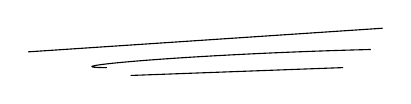
\begin{tikzpicture}[x=1cm,y=1cm]
\draw (0,.4)--(4.5,.7);
\draw (4.35,.43) .. controls (2,.37) and (.2,.2) .. (1,.2);
\draw (1.3,.1)--(4,.2);
\end{tikzpicture}}

\diagram{\begin{tikzcd}
\deleted{A}\arrow[r,hook]\arrow[rr,bend right=28] &
\deleted{M} & \deleted{M'}\arrow[l,"\deleted{f^*}"']
\end{tikzcd}}

\deleted{$f^*$ commute aux $\varprojlim$}

\deleted{$f_!$ existe alors, si on suppose que $\forall$ foncteur sur $M'$
qui commute aux $\varprojlim$ est représentable --- à vérifier des conditions
qui l'assurent, quitte parfois à faire des hyp. d'admissibilité sur $f^*$.
Mais va-t-on supposer que $f_!$ applique $M_{\mathrm{as}}$ dans $M'_{\mathrm{as}}$?}

\diagram{\begin{tikzcd}
\deleted{M}\arrow[r,shift left,"\deleted{f_!}"] &
\deleted{M'}\arrow[l,shift left,"\deleted{f^*}"]
\end{tikzcd}}

\deleted{Si $f:A\unsure{-|\longrightarrow} B$ asphérique, a-t-on
\[
f_!(\widehat A_{\mathrm{as}})\subset\widehat B_{\mathrm{as}}\ ?
\]
Par exemple prenons $B$ ponctuelle, \uline{$A$ cat. asph},}

\figure{\begin{tikzpicture}[x=1cm,y=1cm]
\draw (1.1,7.3) .. controls (1.5,4.6) and (3.2,1.2) .. (4.3,0.5);
\draw (4.8,7.3) .. controls (5.8,4.5) and (7.7,1.8) .. (7.6,1.2);
\draw (0,4.4) .. controls (.2,2.8) and (1.7,.4) .. (2.6,-.3);
\end{tikzpicture}}
\cotefile{115}
\scanpage{2}
% archive foliation: 1
% Pale mirrored printer characters show through from the reverse.
``Correspondances'' fonctorielles

Dualité des topos
\scanpage{3}
% archive foliation: 2
\[
H_A^{\deleted{\unsure{*}}}
\bigl(f^*(\underset{\substack{\vert\\b^\circ}}{\Psi_*}),
\underset{\substack{\vert\\a^\circ}}{\Phi^{\unsure{*|\circ}}}\bigr)
\overset{?}{\simeq}
H_B\bigl(\Psi_*,f^\circ_!(\Phi^*)\bigr)
\]
\[
\operatorname{Hom}_B(b,f(a))=
\operatorname{Hom}_{\widehat B}(b,f_{\unsure{!}}(a))
\overset{?}{\simeq}\operatorname{Hom}_{\widehat A}(\unsure{f^*b},a)
\]
\[
H_A\bigl(\underset{\wedge}{f^*(b)},\underset{\substack{\vert\\\vee}}a\bigr)
\simeq H_B\bigl(\underset{\wedge}{b},\underset{\vee}{f^\circ(a)}\bigr)
=\operatorname{Hom}_B(b,f(a))
\]
\[
\unsure{\Vert}\quad\inserted{\overset{\wedge\quad\vee}{\operatorname{Hom}}}
\quad\deleted{\operatorname{Hom}_{\widehat A}(f^*(b),a)=\operatorname{Hom}}
\]
\[
f^*(b)=\varinjlim_{a'\text{ ds }A/b}a'^{\unsure{\circ}}
\]
\[
\unsure{\forall|H_A}\ \varprojlim_{a'\text{ ds }A/b}\operatorname{Hom}_A(a',a)
\]

% The following draft is written in the opposite orientation and crossed by two long diagonal strokes.
\diagram{\begin{array}{l}
\deleted{\widehat B^\circ\unsure{\longrightarrow|{-}}\widehat A}\quad
\left\{\deleted{\unsure{B\times}}\ \deleted{\widehat B^\circ\times}\right.\\
\deleted{B^\vee\unsure{\longrightarrow|{-}}\widehat A}\\
\deleted{\widehat A^\circ\unsure{\longrightarrow|{-}}\widehat B}\\
\deleted{A^\vee\unsure{\longrightarrow|{-}}\widehat B}
\end{array}}

\figure{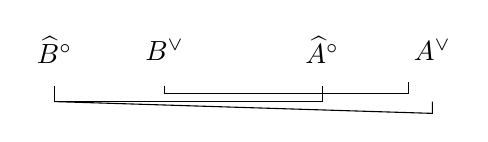
\begin{tikzpicture}[x=1cm,y=1cm]
\node at (0,1) {$\deleted{\widehat B^\circ}$};
\node at (1.4,1) {$\deleted{B^\vee}$};
\node at (3.4,1) {$\deleted{\widehat A^{\unsure{\circ}}}$};
\node at (4.8,1) {$\deleted{A^\vee}$};
\draw (0,.55)--(0,.35)--(3.4,.35)--(3.4,.55);
\draw (1.4,.55)--(1.4,.45)--(4.5,.45)--(4.5,.6);
\draw (0,.35)--(4.8,.2)--(4.8,.35);
\end{tikzpicture}}

\diagram{\begin{array}{c|c}
\deleted{\widehat A^\circ}&\deleted{\widehat B^\circ}\\
\deleted{A^\vee}&\deleted{B^\vee}
\end{array}}

\diagram{\begin{tikzcd}[column sep=large,row sep=small]
\deleted{\widehat B^\circ}\arrow[r,"\deleted{!}"] & \deleted{\widehat A}
& \deleted{\widehat B^\circ\times\widehat A^\circ}\arrow[r,"\deleted{!!}"]
& \deleted{\operatorname{Ens}}\arrow[dddd,no head,bend left=20]\\
&&\deleted{\widehat B^\circ\times A^\vee}\arrow[r,"\deleted{!}","\deleted{!}"']
&\deleted{\operatorname{Ens}}\arrow[ddddd,no head,bend left=48]\\
\deleted{B^\vee}\arrow[r,"\deleted{!}"'] &\deleted{\widehat A}
&\deleted{B^\vee\times\widehat A^\circ}\arrow[r,"\deleted{!}","\deleted{!}"']
&\deleted{\operatorname{Ens}}\arrow[ddd,no head,bend left=35]\\
&&\deleted{B^\vee\times A^\vee}\arrow[r,"\deleted{!!}"']
&\deleted{\operatorname{Ens}}\arrow[dddd,no head,bend left=65]\\
\deleted{\widehat A^\circ}\arrow[r,"\deleted{!}"] &\deleted{\widehat B}
&\deleted{\widehat A^\circ\times\widehat B^\circ}\arrow[r,"\deleted{!!}"]
&\deleted{\operatorname{Ens}}\\
&&\deleted{\widehat A^\circ\times B^\vee}\arrow[r,"\deleted{!}","\deleted{!}"']
&\deleted{\operatorname{Ens}}\\
\deleted{A^\vee}\arrow[r,"\deleted{!}"'] &\deleted{\widehat B}
&\deleted{A^\vee\times\widehat B^\circ}\arrow[r,"\deleted{!}","\deleted{!}"']
&\deleted{\operatorname{Ens}}\\
&&\deleted{A^\vee\times B^\vee}\arrow[r,"\deleted{!!}"']
&\deleted{\operatorname{Ens}}
\end{tikzcd}}
\figure{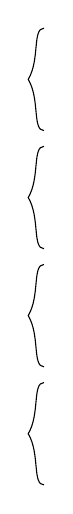
\begin{tikzpicture}
\foreach \y in {0,1.5,3,4.5}{\draw (0,\y+.65) .. controls (-.15,\y+.65) and (-.05,\y+.25) .. (-.2,\y)
 .. controls (-.05,\y-.25) and (-.15,\y-.65) .. (0,\y-.65);}
\end{tikzpicture}}

\margin{\deleted{$\underline{\operatorname{Hom}}(\widehat A^\circ,\unsure{''})$}}
\margin{\deleted{\uuline{Hom}\unsure{.}}}
\diagram{\begin{array}{l|ll}
&\deleted{\widehat A}\ \deleted{\text{contr}}&\deleted{\text{contr }\widehat B}\\
&\deleted{A^\vee}\ \deleted{\text{co}}&\deleted{B}
\end{array}}

\diagram{\begin{tikzcd}[column sep=small,row sep=small]
&&{}&&&&{}\\
{}&\deleted{\widehat A^\circ-\widehat B}\arrow[ddl,no head]\arrow[dr,no head]
&&\deleted{\widehat B^\circ-\widehat A}\arrow[dl,no head]\arrow[drrr,no head]&{}&&\\
&&\deleted{\widehat A,\widehat B}\arrow[uu,no head]\arrow[dll,no head,"\deleted{\widehat A}"']
\arrow[rrrr,no head,"\deleted{\widehat B}"]&&&&\deleted{A^\vee,\widehat B}\arrow[uu,no head]\arrow[dll,no head,"\deleted{A^\vee}"]\\
\deleted{\widehat A,B^\vee}\arrow[uu,no head]\arrow[rrrr,no head,"\deleted{B^\vee}"']&&&&\deleted{A^\vee,B^\vee}\arrow[uu,no head]&&
\end{tikzcd}}

\figure{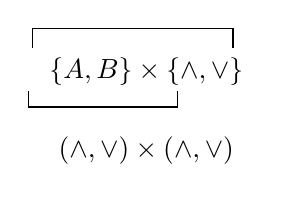
\begin{tikzpicture}[x=1cm,y=1cm]
\node at (1.6,1) {$\deleted{\{A,B\}\times\{\wedge,\vee\}}$};
\node at (1.6,0) {$\deleted{(\unsure{\wedge},\vee)\times(\wedge,\vee)}$};
\draw (.15,1.3)--(.15,1.55)--(2.7,1.55)--(2.7,1.3);
\draw (.1,.75)--(.1,.55)--(2,.55)--(2,.75);
\end{tikzpicture}}

\diagram{\begin{tikzcd}[column sep=small,row sep=large]
&&\deleted{\underline{\operatorname{Hom}}^!(\widehat A^\circ,\widehat B)}\arrow[dll,bend right=20]\arrow[drr,bend left=15]&&\\
\deleted{\underline{\operatorname{Hom}}^{\unsure{!!}}_{\deleted{\unsure{!}}}(\widehat A^\circ,\widehat B^\circ;\operatorname{Ens})}
&&\deleted{\widehat A}\arrow[dd,no head]
&&\deleted{\underline{\operatorname{Hom}}^{\unsure{!}}_{!}(\widehat A^\circ,B^\vee;\operatorname{Ens})}\\
&\deleted{\wedge\wedge}\ \deleted{\unsure{\operatorname{Ens}\ \underline{\operatorname{Hom}}}}
&&\deleted{\wedge\vee}&\unsure{\wr}\arrow[d,no head]\\
\deleted{\underline{\operatorname{Hom}}^!(\widehat B^\circ,\widehat A)}\arrow[uu,bend left=10]\arrow[ddd,bend right=15]
&\deleted{\widehat B}\arrow[r,no head]
&\deleted{\widehat{(A\times B)}}\arrow[r,no head]
&\deleted{B^\vee}
&\deleted{\underline{\operatorname{Hom}}_!(B^\vee,\widehat A)}\arrow[uu,bend right=20]\arrow[ddd,bend left=15]\\
&\deleted{\vee\wedge}
&\deleted{A^\vee}\arrow[u,no head]
&\deleted{\vee\vee}\ \deleted{\unsure{\underline{\operatorname{Hom}}}}&\\
&&&&\\
\deleted{\underline{\operatorname{Hom}}^{\unsure{!}}_{\unsure{!}}(\unsure{A^\vee},\unsure{\widehat B^\circ};\operatorname{Ens})}
&&\deleted{\underline{\operatorname{Hom}}_!(A^\vee,\widehat B)}\arrow[ll]\arrow[rr,bend right=15]
&&\deleted{\underline{\operatorname{Hom}}_{!!}(A^\vee,B^\vee;\operatorname{Ens})}\\
\deleted{\unsure{(\widehat A,\widehat B,\operatorname{Ens})}}&&&&
\end{tikzcd}}

\figure{\begin{tikzpicture}[x=1cm,y=1cm]
\draw (0,5.7)--(12,0.1);
\draw (5.8,0)--(11.7,7.2);
\end{tikzpicture}}

\diagram{\begin{array}{l}
\texttt{//\unsure{PREDONMA|PREDONAA} JOB CNU0049\$NODER=PREDONT} \\
\texttt{/*JOBPARM L=15} \\
\texttt{//COMP EXEC FORTXC,PARM=TERM,REGION=300K} \\
\texttt{//FORT.SYSPRINT DD DSN=\&MESSYS,SPACE=(CYL,4),UNIT=SYSDA,DISP=(MOD,PASS)} \\
\texttt{//FORT.SYSTERM DD DSN=\&MESCOM,SPACE=(CYL,2),UNIT=SYSDA,DISP=(MOD,PASS)} \\
\texttt{//SYSIN DD DSN=CNU1.MODULEF.V33.INTERME1(MEFCONVS),DISP=OLD} \\
\texttt{//CUTR EXEC PGM=CUTTER} \\
\texttt{//STEPLIB DD DSN=CNU2.MODULEF.UTIA,DISP=SHR} \\
\texttt{//TERMINAL DD DSN=\&MESCOM,DISP=(OLD,DELETE)} \\
\texttt{//OBJECT1 DD DSN=\&ORJ,DISP=(OLD,DELETE)} \\
\texttt{//SOURCE1 DD DSN=\&MESSYS,DISP=(OLD,DELETE)} \\
\texttt{//SYSPRINT DD DUMMY} \\
\texttt{//SOURCE2 DD DSN=\&SOURCE,SPACE=(CYL,4),UNIT=SYSDA,DISP=(MOD,PASS)} \\
\texttt{//OBJECT2 DD DSN=\&ORJ2,SPACE=(CYL,3),UNIT=SYSDA,DISP=(MOD,PASS)} \\
\texttt{//UPDT EXEC PGM=UPDATE,COND=(0,NE,CUTR),PARM=NEW} \\
\texttt{//STEPLIB DD DSN=CNU2.MODULEF.UTIA,DISP=SHR} \\
\texttt{//SYSIN DD DSN=\&SOURCE,DISP=(OLD,DELETE)} \\
\texttt{//SYSIN2 DD UNIT=SYSDA,SPACE=(CYL,4)} \\
\texttt{//SYSUT\deleted{\unsure{1}}\inserted{2} DD DSN=CNU2.MODULEF.CONVS,DISP=(,CATLG),SPACE=(TRK,(20,2,35)),} \\
\texttt{// DCB=(RECFM=FB,LRECL=80,BLKSIZE=19040),UNIT=SYSDA,VOL=SER=SYSPPP} \\
\texttt{//SYSPRINT DD SYSOUT=*} \\
\texttt{//LIEN EXEC FORTXL,COND=(0,NE,CUTR)} \\
\texttt{//LKED.SYSLIN DD DSN=\&ORJ2,DISP=(OLD,DELETE)} \\
\texttt{//LKED.SYSLMOD DD DSN=CNU2.MODULEF.CONV,SPACE=(TRK,(40,4,35)),} \\
\texttt{// DCB=(RECFM=U,BLKSIZE=19040),UNIT=SYSDA,VOL=SER=SYSPPP,DISP=(,CATLG)} \\
\texttt{//FIN EXEC PGM=IEFBR14,COND=((0,EQ,UPDT),(4,GE,LIEN.LKED),EVEN)} \\
\texttt{//SOURCE DD DSN=CNU2.MODULEF.CONVS,DISP=(OLD,DELETE)} \\
\texttt{//MODEX DD DSN=CNU2.MODULEF.CONV,DISP=(OLD,DELETE)} \\
\texttt{//}
\end{array}}

\figure{\begin{tikzpicture}[x=1cm,y=1cm]
\draw[->](0,4.7)--(.5,4.7);
\draw[->](0,2.2)--(.5,2.2);
\draw[->](0,1.2)--(.5,1.2);
\draw[->](0,.8)--(.5,.8);
\draw[->](6.5,2.2)--(6,2.2);
\end{tikzpicture}}
\scanpage{4}
\mspage{\textcircled{1}}
% archive foliation: 3
\margin{Cas $B=A^\circ$, d'où élément canonique
$H=H_A\in\widehat{(A\times A^\circ)}$.
D'où $A\hookrightarrow\widehat A$, $A^\circ\hookrightarrow A^\vee$
(les plongements can)
\[
A^{\vee\circ}\xrightarrow{!}\widehat A,\quad
\widehat A^\circ\xrightarrow{!}A^\vee\quad(\text{comm. aux }\varprojlim)
\]
\[
\widehat A^\circ\times A^{\vee\circ}\xrightarrow{!!}(\operatorname{Ens})
\]
(bif. can. sur $\widehat A,A^\vee$)
\inserted{i.e. faisceaux sur $A^\vee$ repr. $\widehat A$;
\unsure{i.e. ds} $\widehat A$ repr. $A^\vee$}
(et $\widehat A\unsure{\longrightarrow|{-}}\widehat A$ et
$A^\vee\unsure{\longrightarrow|{-}}A^\vee$ sont les identités)
\[
\widehat A\simeq\underline{\operatorname{Hom}}^!(\widehat A^\circ,\operatorname{Ens})
\simeq\underline{\operatorname{Hom}}_!(A^\vee,\operatorname{Ens})
\]
\[
A^\vee\simeq\underline{\operatorname{Hom}}^!(A^{\vee\circ},\operatorname{Ens})
\simeq\underline{\operatorname{Hom}}_!(\widehat A,\operatorname{Ens})
\]
et \unsure{item|idem} pour $B$}

\figure{\begin{tikzpicture}[x=1cm,y=1cm]
\draw (0,0) .. controls (1.2,1) and (1,2.5) .. (2.4,2.7)
 .. controls (3.4,3) and (3.4,3.5) .. (4.2,3.5)
 .. controls (5.1,3.8) and (5.2,5) .. (6,5.8);
\end{tikzpicture}}

\margin{$\underline{\operatorname{Hom}}_!$: sous-cat. pleine de $\underline{\operatorname{Hom}}$
formée des foncteurs commutant aux $\varinjlim$.

$\underline{\operatorname{Hom}}^!$: sous-cat. pleine de $\underline{\operatorname{Hom}}$
formée des foncteurs commutant aux $\varprojlim$.}

\diagram{\begin{tikzcd}[column sep=small,row sep=large]
&&\widehat{(A\times B)}\arrow[dl,no head,"\simeq"']\arrow[dr,no head,"\simeq"]&&\\
&\underline{\operatorname{Hom}}(B^\circ,\underline{\widehat A})
&&\underline{\operatorname{Hom}}(A^\circ,\widehat B)&\\
\underline{\operatorname{Hom}}_!(B^\vee,\widehat A)\arrow[ur,"\simeq"]
&\underline{\operatorname{Hom}}^!(\widehat B^\circ,\underline{\widehat A})\arrow[u,"\simeq"']\arrow[dr,"\simeq"']
&&\underline{\operatorname{Hom}}^!(\widehat A^\circ,\widehat B)\arrow[u,"\simeq"]\arrow[dl,"\simeq"]
&\underline{\operatorname{Hom}}_!(A^\vee,\widehat B)\arrow[ul,"\simeq"']\arrow[d,no head,"\simeq"]\\
\underline{\operatorname{Hom}}_{!!}(A^\vee\times B^\vee,(\operatorname{Ens}))\Big]\arrow[u,"\simeq"]
&&\begin{gathered}\underline{\operatorname{Hom}}^{!!}(\widehat A^\circ\times\widehat B^\circ,(\operatorname{Ens}))\\=\operatorname{Bifais}(\widehat A,\widehat B)\end{gathered}
&&\underline{\operatorname{Hom}}_{!!}(A^\vee\times B^\vee,(\operatorname{Ens}))
\end{tikzcd}}

\diagram{\begin{tikzcd}
&A\times B\arrow[dl,"p_B"']\arrow[dr,"p_A"]&\\
A\arrow[dr,no head,"q_A"']&&B\arrow[dl,"q_B"]\\
&e&
\end{tikzcd}}

\[
\left\{\begin{aligned}
\underline{\operatorname{Hom}}_A(X,Y)&\overset{\mathrm{def}}=p_{B*}\underline{\operatorname{Hom}}_{A\times B}(X,Y)\\
\underline{\operatorname{Hom}}_B(X,Y)&\overset{\mathrm{def}}=p_{A*}\underline{\operatorname{Hom}}_{A\times B}(X,Y)\\
\operatorname{Hom}_{A\times B}(X,Y)&\simeq\Gamma_{A\times B}\underline{\operatorname{Hom}}_{A\times B}(X,Y)
\simeq\Gamma_A\underline{\operatorname{Hom}}_A(X,Y)
\simeq\Gamma_B\underline{\operatorname{Hom}}_B(X,Y)
\end{aligned}\right.
\]
\margin{$X,Y\in\operatorname{Ob}\widehat{(A\times B)}$}

\[
\left\{\begin{aligned}
{}^sX(L)&=\underline{\operatorname{Hom}}_B(p_B^*L,X)
=p_{A*}\underline{\operatorname{Hom}}_{A\times B}(p_B^*L,X)\\
{}^dX(M)&=\underline{\operatorname{Hom}}_A(p_A^*M,X)
=p_{B*}\underline{\operatorname{Hom}}_{A\times B}(p_A^*M,X)\\
X(L,M)&=\operatorname{Hom}_{A\times B}(L\boxtimes M,X)
\simeq\operatorname{Hom}_{\widehat A}(L,{}^dX(M))
\simeq\operatorname{Hom}_{\widehat B}(M,{}^sX(L))
\end{aligned}\right.
\]
\margin{$L\in\operatorname{Ob}\widehat A$\quad$M\in\operatorname{Ob}\widehat B$}
où $L\boxtimes M=p_B^*L\times p_A^*M$.

\inserted{Ces formules sont particulièrement intéressantes pour
$L=a\in\operatorname{Ob}A$ $M=b\in\operatorname{Ob}B$}

Soit $X$, définissant $B^\circ\longrightarrow\widehat A$
(savoir $b\longmapsto{}^dX(b)=\underline{\operatorname{Hom}}_B(p_B^*(L),X)$),
\unsure{composons} avec $\widehat A\longrightarrow\operatorname{Ens}$ défini
par un $L_0\in\operatorname{Ob}\widehat A$, par
$L'\longmapsto\operatorname{Hom}(L_0,L')$, on trouve
$B^\circ\longrightarrow\operatorname{Ens}$: i.e.
\deleted{$\unsure{b\longmapsto\operatorname{Hom}(L_0|b\longmapsto\operatorname{Hom}_{\widehat A}}$}
\inserted{$b\longmapsto\operatorname{Hom}_{\widehat A}(L_0,{}^dX(b))$, i.e.}
un élément de $\widehat B$, qui n'est autre que
$\underline{\operatorname{Hom}}_B(p_B^*\unsure{L_0},X)={}^sX(L_0)$.
Interprétation duale pour ${}^dX(M)$.

\[
(L,M)\longmapsto L\boxtimes M:\quad
\widehat A\times\widehat B\longrightarrow\widehat{(A\times B)}
\]
est pleinement fidèle,
\diagram{\begin{tikzcd}
\widehat{(A\times B)}\arrow[d,"\unsure{\simeq}"]\\
\underline{\operatorname{Hom}}^{!!}(\widehat A^\circ\times\widehat B^\circ,\operatorname{Ens})
\subset\widehat{(\widehat A\times\widehat B)}
\end{tikzcd}}
le composé est le foncteur canonique dit ``de Yoneda'' pour
$\widehat A\times\widehat B$.

\[
\operatorname{Hom}_{A\times B}
(\unsure{L'^{\xi}|L^{\xi}}\boxtimes\unsure{M'^{\xi}|M^{\xi}},
L^{\unsure{\xi|\sharp}}\boxtimes M^{\unsure{\xi|\sharp}})
\simeq
(L^{\unsure{\xi|\sharp}}\boxtimes M^{\unsure{\xi|\sharp}})
(L'^{\unsure{\xi|\sharp}}\boxtimes M'^{\unsure{\xi|\sharp}})
\xleftarrow{\sim}
\operatorname{Hom}_{\widehat A}(L'^{\unsure{\xi|\sharp}},L^{\unsure{\xi|\sharp}})
\times\operatorname{Hom}_{\widehat B}(M'^{\unsure{\xi|\sharp}},M^{\unsure{\xi|\sharp}})
\]
\[
\underline{\operatorname{Hom}}_{A\times B}
(L'^{\unsure{\xi|\sharp}}\boxtimes M'^{\unsure{\xi|\sharp}},L^{\unsure{\xi|\sharp}}\boxtimes M^{\unsure{\xi|\sharp}})
\simeq\underline{\operatorname{Hom}}_{\widehat A}(L'^{\unsure{\xi|\sharp}},L^{\unsure{\xi|\sharp}})
\boxtimes\underline{\operatorname{Hom}}_{\widehat B}(M'^{\unsure{\xi|\sharp}},M^{\unsure{\xi|\sharp}})
\]
\margin{p.ex.}
\[
\underline{\operatorname{Hom}}_{A\times B}
(L^{\unsure{\xi'}}\boxtimes M',
\underbrace{L^{\unsure{\xi|\sharp}}\boxtimes e_{\widehat B}}_{p_B^*L^{\unsure{\xi|\sharp}}})
\simeq
\underbrace{\underline{\operatorname{Hom}}_{\widehat A}(L',L^{\unsure{\xi|\sharp}})\boxtimes e_{\widehat B}}_{p_B^*\underline{\operatorname{Hom}}_{\widehat A}(L,L')}
\]
\margin{en particulier faisant $L'=e_{\widehat A}$ et changeant $M'$ en $M$}
\[
\underline{\operatorname{Hom}}_{A\times B}(p_A^*(M),p_B^*L)
\xleftarrow{\sim}p_B^*L
\]
(la flèche étant la flèche canonique
$\underline{\operatorname{Hom}}(\alpha,\beta)\longleftarrow\beta$)

Posant $X^M\overset{\mathrm{def}}=\underline{\operatorname{Hom}}_{A\times B}(p_A^*M,X)$,
on trouve donc $(p_B^*L)^M\simeq p_B^*L$

\unsure{p}
\scanpage{5}
% archive foliation: 4
\diagram{\begin{array}{l}
\texttt{PPPPPPPPPPP\ \ \ RRRRRRRRRRR\ \ \ EEEEEEEEEEEE\ \ DDDDDDDDD\ \ \ \ \ OOOOOOOOOOOO\ \ NN\ \ \ \ \ \ \ \ NN\ \ TTTTTTTTTTTT} \\
\texttt{PPPPPPPPPPPP\ \ RRRRRRRRRRRR\ \ EEEEEEEEEEEE\ \ DDDDDDDDDD\ \ \ \ OOOOOOOOOOOO\ \ NNN\ \ \ \ \ \ \ NN\ \ TTTTTTTTTTTT} \\
\texttt{PP\ \ \ \ \ \ \ \ PP\ \ RR\ \ \ \ \ \ \ \ RR\ \ EE\ \ \ \ \ \ \ \ \ \ \ \ DD\ \ \ \ \ \ \ DD\ \ \ OO\ \ \ \ \ \ \ \ OO\ \ NNNN\ \ \ \ \ \ NN\ \ \ \ \ \ \ TT} \\
\texttt{PP\ \ \ \ \ \ \ \ PP\ \ RR\ \ \ \ \ \ \ \ RR\ \ EE\ \ \ \ \ \ \ \ \ \ \ \ DD\ \ \ \ \ \ \ \ DD\ \ OO\ \ \ \ \ \ \ \ OO\ \ NN\ NN\ \ \ \ \ NN\ \ \ \ \ \ \ TT} \\
\texttt{PP\ \ \ \ \ \ \ \ PP\ \ RR\ \ \ \ \ \ \ \ RR\ \ EE\ \ \ \ \ \ \ \ \ \ \ \ DD\ \ \ \ \ \ \ \ DD\ \ OO\ \ \ \ \ \ \ \ OO\ \ NN\ \ NN\ \ \ \ NN\ \ \ \ \ \ \ TT} \\
\texttt{PPPPPPPPPPPP\ \ RRRRRRRRRRRR\ \ EEEEEEEE\ \ \ \ \ \ DD\ \ \ \ \ \ \ \ DD\ \ OO\ \ \ \ \ \ \ \ OO\ \ NN\ \ \ NN\ \ \ NN\ \ \ \ \ \ \ TT} \\
\texttt{PPPPPPPPPPP\ \ \ RRRRRRRRRRR\ \ \ EEEEEEEE\ \ \ \ \ \ DD\ \ \ \ \ \ \ \ DD\ \ OO\ \ \ \ \ \ \ \ OO\ \ NN\ \ \ \ NN\ \ NN\ \ \ \ \ \ \ TT} \\
\texttt{PP\ \ \ \ \ \ \ \ \ \ \ \ RR\ \ \ \ RR\ \ \ \ \ \ EE\ \ \ \ \ \ \ \ \ \ \ \ DD\ \ \ \ \ \ \ \ DD\ \ OO\ \ \ \ \ \ \ \ OO\ \ NN\ \ \ \ \ NN\ NN\ \ \ \ \ \ \ TT} \\
\texttt{PP\ \ \ \ \ \ \ \ \ \ \ \ RR\ \ \ \ \ RR\ \ \ \ \ EE\ \ \ \ \ \ \ \ \ \ \ \ DD\ \ \ \ \ \ \ \ DD\ \ OO\ \ \ \ \ \ \ \ OO\ \ NN\ \ \ \ \ \ NNNN\ \ \ \ \ \ \ TT} \\
\texttt{PP\ \ \ \ \ \ \ \ \ \ \ \ RR\ \ \ \ \ \ RR\ \ \ \ EE\ \ \ \ \ \ \ \ \ \ \ \ DD\ \ \ \ \ \ \ DD\ \ \ OO\ \ \ \ \ \ \ \ OO\ \ NN\ \ \ \ \ \ \ NNN\ \ \ \ \ \ \ TT} \\
\texttt{PP\ \ \ \ \ \ \ \ \ \ \ \ RR\ \ \ \ \ \ \ RR\ \ \ EEEEEEEEEEEE\ \ DDDDDDDDDD\ \ \ \ OOOOOOOOOOOO\ \ NN\ \ \ \ \ \ \ \ NN\ \ \ \ \ \ \ TT} \\
\texttt{PP\ \ \ \ \ \ \ \ \ \ \ \ RR\ \ \ \ \ \ \ \ RR\ \ EEEEEEEEEEEE\ \ DDDDDDDDD\ \ \ \ \ OOOOOOOOOOOO\ \ NN\ \ \ \ \ \ \ \ \ N\ \ \ \ \ \ \ TT}
\end{array}}

\texttt{****A END JOB 3 PREDONT - CRAY OUTPUT - ROOM 11.24.23 AM 02 JUN 82 R6.PR1 SYS JES2 JOB 3 END A****}

\texttt{****A END JOB 3 PREDONT - CRAY OUTPUT - ROOM 11.24.23 AM 02 JUN 82 R6.PR1 SYS JES2 JOB 3 END A****}

\texttt{****A END JOB 3 PREDONT - CRAY OUTPUT - ROOM 11.24.23 AM 02 JUN 82 R6.PR1 SYS JES2 JOB 3 END A****}

\texttt{****A END JOB 3 PREDONT - CRAY OUTPUT - ROOM 11.24.23 AM 02 JUN 82 R6.PR1 SYS JES2 JOB 3 END A****}

\texttt{****A END JOB 3 PREDONT - CRAY OUTPUT - ROOM 11.24.23 AM 02 JUN 82 R6.PR1 SYS JES2 JOB 3 END A****}

\texttt{****A END JOB 3 PREDONT - CRAY OUTPUT - ROOM 11.24.23 AM 02 JUN 82 R6.PR1 SYS JES2 JOB 3 END A****}
\scanpage{6}
\mspage{\textcircled{2}}
% archive foliation: 5
\diagram{\left.\begin{array}{c}A^\circ,\widehat A^\circ,A^\vee\\B^\circ,\widehat B^\circ,B^\vee\end{array}\right|
\begin{tikzcd}[column sep=small,row sep=small]{}\arrow[dr]&{}\\{}\arrow[ur]&{}\end{tikzcd}
\left|\begin{array}{c}\widehat A\\\widehat B\end{array}\right.}\quad(6\text{ Cas})
\[
\left|\widehat A^\circ\ \underset{\unsure{\rightarrow}}{\text{ou}}\ A^\vee\right|
\times\left|\widehat B^\circ\ \text{ou}\ B^\vee\right|\longrightarrow\mathrm{Ens}
\qquad(4\text{ Cas})
\]
\uline{NB}
\diagram{\begin{tikzcd}[row sep=small]
\widehat A^{\circ\unsure{-}}&&A^\vee\\
&A^\circ\arrow[ul,hook]\arrow[ur,hook]&
\end{tikzcd}}
\diagram{\begin{tikzcd}[row sep=small]
\widehat B^\circ&&B^\vee\\
&B^\circ\arrow[ul,hook]\arrow[ur,hook]&
\end{tikzcd}}

\margin{$(\widehat B\rightarrow)$}
\margin{\figure{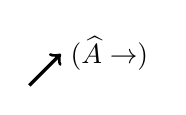
\begin{tikzpicture}\draw[->,very thick](0,0)--(.4,.4);\node[anchor=west] at (.4,.4){$(\widehat A\rightarrow)$};\end{tikzpicture}}}
\diagram{\begin{tikzcd}[column sep=small,row sep=large]
&&&\underline{\mathrm{Hom}}^{!!}(\widehat A^\circ,\widehat B^\circ;\mathrm{Ens})&&&\\
&\underline{\mathrm{Hom}}^!(\widehat B^\circ,\widehat A)\arrow[urr,bend left=15]\arrow[ddl,bend right=15]&&&&\underline{\mathrm{Hom}}^!(\widehat A^\circ,\widehat B)\arrow[ull,bend right=15]\arrow[ddr,bend left=15]\arrow[dl] &\\
&&\underline{\mathrm{Hom}}(B^\circ,\widehat A)\arrow[ul]&&\underline{\mathrm{Hom}}(A^\circ,\widehat B)&&\\
\underline{\mathrm{Hom}}_!^!(A^\vee,\widehat B^\circ;\mathrm{Ens})&&&
\begin{gathered}(A\times B)^\wedge\\=\underline{\mathrm{Hom}}(A^\circ,B^\circ;\mathrm{Ens})\end{gathered}
\arrow[ul]\arrow[ur]\arrow[dl]\arrow[dr]
\arrow[uuu,no head,"\wedge\wedge" description]
\arrow[lll,no head,"\vee\wedge" description]
\arrow[rrr,no head,"\wedge\vee" description]
\arrow[ddd,no head,"\vee\vee" description]
&&&\underline{\mathrm{Hom}}^!_!(\widehat A^\circ,B^\vee;\mathrm{Ens})\\
&&\underline{\mathrm{Hom}}(A^\circ,\widehat B)\arrow[dl]&&\underline{\mathrm{Hom}}(B^\circ,\widehat A)\arrow[dr]&&\\
&\underline{\mathrm{Hom}}_!(A^\vee,\widehat B)\arrow[uul,bend left=15]\arrow[drr,bend right=15]&&&&\underline{\mathrm{Hom}}_!(B^\vee,\widehat A)\arrow[uur,bend right=15]\arrow[dll,bend left=15]&\\
&&&\underline{\mathrm{Hom}}_{!!}(A^\vee,B^\vee;\mathrm{Ens})&&&
\end{tikzcd}}
\margin{$(A^\vee\rightarrow)$\qquad$(B^\vee\rightarrow)$}
Toutes les flèches du diagramme sont des équivalences de catégories

$I$ ens d'indices

$(A_i)_{i\in I}$ famille de (petites) catégories
\figure{\begin{tikzpicture}\draw (0,0)--(0,1.4);\end{tikzpicture}}

Si $I'\subset I$, on pose
\[
A_{I'}=\prod_{i'\in I'}A_{i'}
\]
\[
I=\coprod_{j\in J}I_j,\quad J=J^+\amalg J^-\qquad
I^+=\coprod_{j\in J^+}I_{j^+},\quad I^-=\coprod_{j\in J^-}I_{j^-}
\]
Je suppose $I,J$ finis pour ``play safe''.
\figure{\begin{tikzpicture}\draw(0,0)--(3,1.5);\end{tikzpicture}}
\diagram{\begin{tikzcd}[column sep=large,row sep=large]
&\widehat A_I\arrow[d,"\unsure{\varphi}"',"\simeq"]&\\
&\underline{\mathrm{Hom}}^{\deleted{\unsure{!}}!}_!\left(
\prod_{j^-\in J^-}A_{I_{j^-}}^\vee,
\prod_{j^+\in J^+}A_{I_{j^+}}^{\wedge\circ};\mathrm{Ens}\right)
\arrow[dl,"\approx"']\arrow[dr,"\approx"]&\\
\underline{\mathrm{Hom}}_!\left(\prod_{j^-\in J^-}A_{I_{j^-}}^\vee,\widehat A_{I^+}\right)
&&\underline{\mathrm{Hom}}^!\left(\prod_{j^+\in J^+}A_{I_{j^+}}^{\wedge\circ},\widehat A_{I^-}\right)
\end{tikzcd}}
\scanpage{7}
% archive foliation: 6
\diagram{\begin{array}{l}
\texttt{\ \ \ \ \ \ \ \ \ \ \ 00000000\ \ \ \ \ \ 00000000\ \ \ \ \ \ 00000000\ \ \ \ \ \ 00000000} \\
\texttt{\ \ \ \ \ \ \ \ \ 0000000000\ \ \ \ 0000000000\ \ \ \ 0000000000\ \ \ \ 0000000000} \\
\texttt{\ \ \ \ \ \ \ 00\ \ \ \ \ \ 0000\ \ 00\ \ \ \ \ \ 0000\ \ 00\ \ \ \ \ \ 0000\ \ 00\ \ \ \ \ \ 0000} \\
\texttt{\ \ \ \ \ \ 00\ \ \ \ \ 00\ 00\ \ 00\ \ \ \ \ 00\ 00\ \ 00\ \ \ \ \ 00\ 00\ \ 00\ \ \ \ \ 00\ 00} \\
\texttt{\ \ \ \ \ 00\ \ \ \ 00\ \ 00\ \ 00\ \ \ \ 00\ \ 00\ \ 00\ \ \ \ 00\ \ 00\ \ 00\ \ \ \ 00\ \ 00} \\
\texttt{\ \ \ \ 00\ \ \ 00\ \ \ 00\ \ 00\ \ \ 00\ \ \ 00\ \ 00\ \ \ 00\ \ \ 00\ \ 00\ \ \ 00\ \ \ 00} \\
\texttt{\ \ \ 00\ \ 00\ \ \ \ 00\ \ 00\ \ 00\ \ \ \ 00\ \ 00\ \ 00\ \ \ \ 00\ \ 00\ \ 00\ \ \ \ 00} \\
\texttt{\ \ 00\ 00\ \ \ \ \ 00\ \ 00\ 00\ \ \ \ \ 00\ \ 00\ 00\ \ \ \ \ 00\ \ 00\ 00\ \ \ \ \ 00} \\
\texttt{\ 0000\ \ \ \ \ \ 00\ \ 0000\ \ \ \ \ \ 00\ \ 0000\ \ \ \ \ \ 00\ \ 0000\ \ \ \ \ \ 00} \\
\texttt{000\ \ \ \ \ \ \ 00\ \ 000\ \ \ \ \ \ \ 00\ \ 000\ \ \ \ \ \ \ 00\ \ 000\ \ \ \ \ \ \ 00} \\
\texttt{0000000000\ \ \ \ 0000000000\ \ \ \ 0000000000\ \ \ \ 0000000000} \\
\texttt{00000000\ \ \ \ \ \ 00000000\ \ \ \ \ \ 00000000\ \ \ \ \ \ 00000000}
\end{array}}

\figure{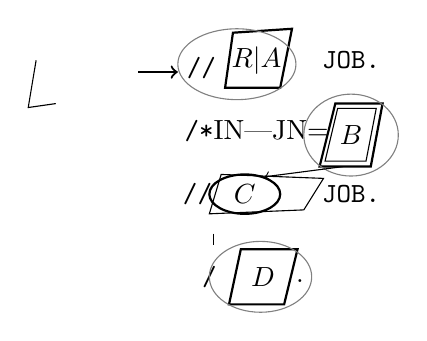
\begin{tikzpicture}[x=1cm,y=1cm]
\draw[thin](-2,0.3)--(-2.1,-.3)--(-1.75,-.25);
\draw[->,thick](-.7,.15)--(-.2,.15);
\node at (.1,.2){\texttt{//}};
\draw[thick](.4,-.05)--(1.1,-.05)--(1.25,.7)--(.5,.65)--cycle;
\node at (.8,.3){$\unsure{R|A}$};\node at (2,.3){\texttt{JOB.}};
\draw[gray,thin](.55,.25) ellipse(.75 and .45);
\node at (.8,-.6){\texttt{/*}\unsure{IN|JN}$=$};
\draw[thick](1.6,-1.05)--(2.25,-1.05)--(2.4,-.25)--(1.8,-.25)--cycle;
\draw[thin](1.67,-.98)--(2.19,-.98)--(2.32,-.31)--(1.83,-.31)--cycle;
\node at (2,-.65){$B$};\draw[gray,thin](2,-.65) ellipse(.6 and .52);
\node at (.05,-1.4){\texttt{//}};\node at (.65,-1.4){$C$};\node at (2,-1.4){\texttt{JOB.}};
\draw[thick](.65,-1.4) ellipse(.45 and .25);
\draw[thin](.35,-1.15)--(1.65,-1.2)--(1.4,-1.6)--(.2,-1.65)--cycle;
\draw[->,thin](1.9,-1.05)--(.9,-1.18);
\draw[thin](.25,-1.9)--(.25,-2.05);
\node at (.2,-2.45){\texttt{/}};
\draw[thick](.45,-2.8)--(1.15,-2.8)--(1.32,-2.1)--(.6,-2.1)--cycle;
\node at (.88,-2.45){$D$};\node at (1.35,-2.5){.};
\draw[gray,thin](.85,-2.45) ellipse(.65 and .45);
\end{tikzpicture}}
\diagram{\begin{array}{l}
\texttt{PPPPPPPPPPP\ \ \ RRRRRRRRRRR\ \ \ EEEEEEEEEEEE\ \ DDDDDDDDD\ \ \ \ \ OOOOOOOOOOOO\ \ NN\ \ \ \ \ \ \ \ NN\ \ TTTTTTTTTTTT\ \ \ AAAAAAAAAA} \\
\texttt{PPPPPPPPPPPP\ \ RRRRRRRRRRRR\ \ EEEEEEEEEEEE\ \ DDDDDDDDDD\ \ \ \ OOOOOOOOOOOO\ \ NNN\ \ \ \ \ \ \ NN\ \ TTTTTTTTTTTT\ \ AAAAAAAAAAAA} \\
\texttt{PP\ \ \ \ \ \ \ \ PP\ \ RR\ \ \ \ \ \ \ \ RR\ \ EE\ \ \ \ \ \ \ \ \ \ \ \ DD\ \ \ \ \ \ \ DD\ \ \ OO\ \ \ \ \ \ \ \ OO\ \ NNNN\ \ \ \ \ \ NN\ \ \ \ \ \ \ TT\ \ \ \ \ \ \ AA\ \ \ \ \ \ \ \ AA} \\
\texttt{PP\ \ \ \ \ \ \ \ PP\ \ RR\ \ \ \ \ \ \ \ RR\ \ EE\ \ \ \ \ \ \ \ \ \ \ \ DD\ \ \ \ \ \ \ \ DD\ \ OO\ \ \ \ \ \ \ \ OO\ \ NN\ NN\ \ \ \ \ NN\ \ \ \ \ \ \ TT\ \ \ \ \ \ \ AA\ \ \ \ \ \ \ \ AA} \\
\texttt{PP\ \ \ \ \ \ \ \ PP\ \ RR\ \ \ \ \ \ \ \ RR\ \ EE\ \ \ \ \ \ \ \ \ \ \ \ DD\ \ \ \ \ \ \ \ DD\ \ OO\ \ \ \ \ \ \ \ OO\ \ NN\ \ NN\ \ \ \ NN\ \ \ \ \ \ \ TT\ \ \ \ \ \ \ AA\ \ \ \ \ \ \ \ AA} \\
\texttt{PPPPPPPPPPPP\ \ RRRRRRRRRRRR\ \ EEEEEEEE\ \ \ \ \ \ DD\ \ \ \ \ \ \ \ DD\ \ OO\ \ \ \ \ \ \ \ OO\ \ NN\ \ \ NN\ \ \ NN\ \ \ \ \ \ \ TT\ \ \ \ \ \ \ AAAAAAAAAAAA} \\
\texttt{PPPPPPPPPPP\ \ \ RRRRRRRRRRR\ \ \ EEEEEEEE\ \ \ \ \ \ DD\ \ \ \ \ \ \ \ DD\ \ OO\ \ \ \ \ \ \ \ OO\ \ NN\ \ \ \ NN\ \ NN\ \ \ \ \ \ \ TT\ \ \ \ \ \ \ AAAAAAAAAAAA} \\
\texttt{PP\ \ \ \ \ \ \ \ \ \ \ \ RR\ \ \ \ RR\ \ \ \ \ \ EE\ \ \ \ \ \ \ \ \ \ \ \ DD\ \ \ \ \ \ \ \ DD\ \ OO\ \ \ \ \ \ \ \ OO\ \ NN\ \ \ \ \ NN\ NN\ \ \ \ \ \ \ TT\ \ \ \ \ \ \ AA\ \ \ \ \ \ \ \ AA} \\
\texttt{PP\ \ \ \ \ \ \ \ \ \ \ \ RR\ \ \ \ \ RR\ \ \ \ \ EE\ \ \ \ \ \ \ \ \ \ \ \ DD\ \ \ \ \ \ \ \ DD\ \ OO\ \ \ \ \ \ \ \ OO\ \ NN\ \ \ \ \ \ NNNN\ \ \ \ \ \ \ TT\ \ \ \ \ \ \ AA\ \ \ \ \ \ \ \ AA} \\
\texttt{PP\ \ \ \ \ \ \ \ \ \ \ \ RR\ \ \ \ \ \ RR\ \ \ \ EE\ \ \ \ \ \ \ \ \ \ \ \ DD\ \ \ \ \ \ \ DD\ \ \ OO\ \ \ \ \ \ \ \ OO\ \ NN\ \ \ \ \ \ \ NNN\ \ \ \ \ \ \ TT\ \ \ \ \ \ \ AA\ \ \ \ \ \ \ \ AA} \\
\texttt{PP\ \ \ \ \ \ \ \ \ \ \ \ RR\ \ \ \ \ \ \ RR\ \ \ EEEEEEEEEEEE\ \ DDDDDDDDDD\ \ \ \ OOOOOOOOOOOO\ \ NN\ \ \ \ \ \ \ \ NN\ \ \ \ \ \ \ TT\ \ \ \ \ \ \ AA\ \ \ \ \ \ \ \ AA} \\
\texttt{PP\ \ \ \ \ \ \ \ \ \ \ \ RR\ \ \ \ \ \ \ \ RR\ \ EEEEEEEEEEEE\ \ DDDDDDDDD\ \ \ \ \ OOOOOOOOOOOO\ \ NN\ \ \ \ \ \ \ \ \ N\ \ \ \ \ \ \ TT\ \ \ \ \ \ \ AA\ \ \ \ \ \ \ \ AA}
\end{array}}
\texttt{****A START JOB 653 PREDONTA ROOM 11.23.37 AM 02 JUN 82 R6.PR1 SYS JES2 JOB 653 START A****}

\texttt{****A START JOB 653 PREDONTA ROOM 11.23.37 AM 02 JUN 82 R6.PR1 SYS JES2 JOB 653 START A****}

\texttt{****A START JOB 653 PREDONTA ROOM 11.23.37 AM 02 JUN 82 R6.PR1 SYS JES2 JOB 653 START A****}

\texttt{****A START JOB 653 PREDONTA ROOM 11.23.37 AM 02 JUN 82 R6.PR1 SYS JES2 JOB 653 START A****}

\texttt{****A START JOB 653 PREDONTA ROOM 11.23.37 AM 02 JUN 82 R6.PR1 SYS JES2 JOB 653 START A****}

\texttt{****A START JOB 653 PREDONTA ROOM 11.23.37 AM 02 JUN 82 R6.PR1 SYS JES2 JOB 653 START A****}

\texttt{DERNIERE MISE A JOUR DE JOURNAL: 24-05-82}
\scanpage{8}
\mspage{\textcircled{3}}
% archive foliation: 7
\[
\boxed{H_A(\Phi,\Psi)=\mathrm{Hom}_{\widehat A}(\Phi,\psi_A(\Psi))\simeq\mathrm{Hom}_{A^\vee}(\Psi,\varphi_A(\Phi))}
\]
\diagram{\begin{tikzcd}[row sep=tiny,column sep=small]
\Phi&\Psi\\
\mathrm{Ob}\widehat A\arrow[u]&\mathrm{Ob}A^\vee\arrow[u]
\end{tikzcd}}
\margin{\diagram{\boxed{\begin{array}{ccc}
\widehat A^\circ&\xrightarrow{\varphi_A}&A^\vee\\
A^{\vee\circ}&\xrightarrow{\psi_A}&\widehat A\\
\widehat A^\circ\times A^{\vee\circ}&\xrightarrow{H_A}&\mathrm{Ens}
\end{array}}}}

i.e. on a
\diagram{\begin{tikzcd}
A^{\vee\circ}\arrow[r,shift right=1.2ex,no head,"\psi_A"']&\widehat A\arrow[l,shift right=1.2ex,"\varphi_A^\circ"']
\end{tikzcd}}
ou
\diagram{\begin{tikzcd}
A^\vee\arrow[r,shift left=1.2ex,no head,"\psi_A^\circ"]&\widehat A^\circ\arrow[l,shift left=1.2ex,"\varphi_A"]
\end{tikzcd}}
paires de foncteurs adjoints

\uline{NB}

a) \diagram{\begin{tikzcd}[row sep=small]
A^{\vee\circ}\arrow[rr,"\psi_A"]&&\widehat A\\
&A\arrow[ul,hook,"h^A"]\arrow[ur,hook,"h_A"']&
\end{tikzcd}}
commutatif, et $\psi_A$ commute aux $\underset{\leftarrow}{\lim}$
-- ce qui caractérise $\psi_A$ à iso unique près

b) \diagram{\begin{tikzcd}[row sep=small]
A^{\vee\circ}&&\widehat A\arrow[ll,"\varphi_A^\circ"']\\
&A\arrow[ul,hook,"h^A"]\arrow[ur,hook,"h_A"']&
\end{tikzcd}}
commutatif, et $\varphi_A^\circ$ commute aux $\underset{\rightarrow}{\lim}$
et cela caractérise $\varphi_A^\circ$ à iso unique près

\margin{\figure{\begin{tikzpicture}\node[inner sep=3pt] (nb) {\begin{minipage}{.34\linewidth}\uline{NB}
$\left\{\begin{aligned}\varphi_{A^\circ}&=\psi_A\\\psi_{A^\circ}&=\varphi_A\\H_{A^\circ}&={}^sH_A\end{aligned}\right.$ i.e.
$H_{A^\circ}(\Psi,\Phi)=H_A(\Phi,\Psi)$
(fonctoriel en $\Phi,\Psi$)
\unsure{\S}\end{minipage}};\draw (nb.north west)--(nb.north east)--(nb.south east)--(nb.south west);\end{tikzpicture}}}

\[
\boxed{\Phi\xrightarrow{\alpha_\Phi}\psi_A\varphi_A^\circ(\Phi)}\quad\text{dans }\widehat A
\qquad\text{i.e.}\qquad
\Phi\longleftarrow\psi_A^\circ\varphi_A(\Phi)\quad\text{dans }\widehat A^\circ
\]
\[
\Psi\longleftarrow\varphi_A^\circ\psi_A(\Psi)\quad\text{dans }A^{\vee\circ}
\qquad\text{i.e.}\qquad
\boxed{\Psi\xrightarrow{\beta_\Psi}\varphi_A\psi_A^\circ(\Psi)\quad\text{dans }A^\vee}
\]
\unsure{\S} morphismes d'adjonction

iso si $\Phi\in\mathrm{Ob}\,A$ ou $\Psi\in\mathrm{Ob}\,A$

c) \(\boxed{H_A(a,b)=\mathrm{Hom}_A(a,b)}\)
\diagram{\begin{tikzcd}[row sep=tiny,column sep=small]
a\arrow[d]&b\arrow[d]\\
\text{pour }h_A(a)&\text{pour }h^A(b)
\end{tikzcd}}
donc $H_A$ prolonge $\mathrm{Hom}_A$, et est caractérisé à iso unique près par cette propriété,
plus celle que $H_A$ commute aux $\underset{\leftarrow}{\lim}$
\inserted{\[
\left[\begin{aligned}
H_A(\Phi,b)&\simeq\mathrm{Hom}_{\widehat A}(\Phi,b)\\
H_A(a,\Psi)&\simeq\mathrm{Hom}_{A^\vee}(\Psi,a)=\mathrm{Hom}_{A^{\vee\circ}}(a,\Psi)
\end{aligned}\right]
\]}
\figure{
\begin{tikzpicture}\draw[->,double](0,.5)--(-.3,0);\end{tikzpicture}}

\uline{Question} Que peut-on dire des morphismes d'adjonction
$\alpha_\Phi,\beta_\Psi$ ? Iso (si et) seulement si $\Phi$ resp. $\Psi$ est représentable ?

\unsure{Est-ce|Est-on} tjrs une équivalence faible (sans doute pas).

Les foncteurs $\varphi_A$ et $\psi_A$ transforment-ils équiv. faibles en isom ?

Relation aux contractions
\[
\boxed{H^A:\quad(\Phi,\Psi)\longmapsto\Phi\mathbin{\ast_A}\Psi\ ;\quad
\widehat A\times A^\vee\underset{!!}{\longrightarrow}\mathrm{Ens}}
\]
d) \(\boxed{H^A(a,b)\overset{\inserted{\text{ou}}}{=}\mathrm{Hom}_A(b,a)}\)
\diagram{\begin{tikzcd}[row sep=tiny,column sep=small]
a\arrow[d]&b\arrow[d]\\
\text{pour }h_A(a)&\text{pour }h^A(b)
\end{tikzcd}}
et $\unsure{H^A_A|H^A}$ commute aux $\underset{\rightarrow}{\lim}$, ce qui le caractérise à iso. unique près
\[
\deleted{\unsure{\varphi^A}\unsure{H_A(a)}\unsure{\ne|=}}
\qquad\boxed{\begin{aligned}\Phi\ast a&=\Phi(a)\\a\ast\Psi&=\Psi(a)\end{aligned}}
\]
\diagram{\boxed{\begin{array}{ccc}
\widehat A&\xrightarrow[\simeq]{\varphi^A}&\underline{\mathrm{Hom}}_!(A^\vee,\mathrm{Ens})\\
A^\vee&\overset{\psi^A}{\underset{\simeq}{\rule{1.2cm}{.3pt}}}&\underline{\mathrm{Hom}}_!(\widehat A,\mathrm{Ens})
\end{array}}}
\figure{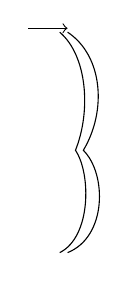
\begin{tikzpicture}\draw(0,0)..controls(.4,.2)and(.4,1)..(.2,1.3)..controls(.4,1.8)and(.35,2.5)..(0,2.8);\draw(.1,0)..controls(.6,.2)and(.6,1)..(.3,1.3)..controls(.6,1.8)and(.55,2.5)..(.1,2.8);\draw[->](-.4,2.85)--(.1,2.85);\end{tikzpicture}}
\unsure{\S}
\[
\boxed{H^A(\Phi,\Psi)=\deleted{\unsure{\Phi}}\varphi^A(\Phi)(\Psi)\simeq\psi^A(\Psi)(\Phi)}
\]

\texttt{/*}\unsure{\texttt{JOBPARM}}\ \unsure{\texttt{********************}}\ \unsure{\texttt{JJ}}\qquad\unsure{\texttt{J0653CNU|J0653GNU}}

\unsure{\texttt{//}}\ \texttt{JOB MSGLEVEL=(1,1)}

\unsure{\texttt{//}}\ \texttt{EXEC CSSBATCH}

\unsure{\texttt{//}}\ \texttt{DD *}
\scanpage{9}
% archive foliation: 8
\[
\left(\prod_{\unsure{j|i}\in I}A_i\right)^\wedge\qquad
A_1^\circ\times A_2^\circ\times\text{---}\times A_n^\circ\longrightarrow\mathrm{Ens}
\qquad A_1\times\cdots\times
\]
\[
\widehat A_1^\circ\times A_2^\vee\times A_3^\vee\times\widehat A_4^\circ\times A_5^\vee\times\cdots\times\widehat A_{n-1}^\circ\times A_n
\]
\deleted{
\[
\deleted{\unsure{A_n}}\quad\mathcal F(\unsure{\mathcal X}_1\times\text{---}\times\unsure{\mathcal X}_n)\deleted{\unsure{\simeq}}\quad
A_1^\circ\times\text{---}\times A_n^\circ\longrightarrow E
\]
\margin{$\unsure{A_n}\quad\deleted{\unsure{\mathcal F}}$}
\[
F\in\mathcal F(\mathcal X_1\times\text{---}\times\mathcal X_n)\qquad
F:A_1^\circ\times\text{---}\times A_n^\circ\longrightarrow\mathrm{Ens}
\]
\[
\widehat A_{\unsure{1}}^\circ\ \text{---}\times\widehat A_n^\circ\mathrel{\rule{.7cm}{.3pt}}\mathrm{Ens}
\]
\[
X_1\otimes X_2\simeq\mathrm{Hom}(X_1^\vee,X_2^\vee;\underline1)
\simeq\mathrm{Hom}(X_1^\vee,X_2)\simeq\mathrm{Hom}(X_2^\vee,X_1)
\]
\[
\begin{aligned}
\mathcal F(X_1,\unsure{\&|\times}X_2)
&\simeq\mathrm{Hom}^{!!}_{\deleted{\unsure{!}}}(\mathcal F(X_1)^\circ,\mathcal F(X_2)^\circ;\mathrm{Ens})
\simeq\mathrm{Hom}^{!}_{\unsure{!}}(\mathcal F(X_1)^\circ,\unsure{\mathcal F}(X_2))
\simeq\mathrm{Hom}^{!}_{\deleted{\unsure{!}}}(\mathcal F(X_2)^\circ,\mathcal F(X_1))\\
&\simeq\mathrm{Hom}_{!!}(\unsure{\mathcal F}(X_1)^\vee,\mathcal F(X_2)^\vee;\mathrm{Ens})
\simeq\mathrm{Hom}_!(\mathcal F(X_1)^\vee,\mathcal F(X_2))
\simeq\mathrm{Hom}_!(\mathcal F(X_2)^\vee,\mathcal F(X_1))\\
&\simeq\mathrm{Hom}(\mathcal F(X_1)^\circ,\mathcal F(X_2)^\vee;\mathrm{Ens})
\end{aligned}
\]
\[
X_I=\overset{\deleted{\unsure{\infty}}}{\prod_{i\in I}}X_j\qquad
X_I=X_{I^+}\times X_{I^-}\simeq\mathrm{Hom}
\]
\[
\mathcal F(\deleted{\unsure{\prod X_i}})\simeq\mathcal F(\prod
\]
\[
I=I^+\amalg I^-
\]
\[
\mathcal F_{\unsure{I|J}}\qquad\widehat X_J\qquad X_J^\vee{}_{\deleted{\unsure{J}}}
\]
\[
\mathcal F(X_J)\qquad\mathcal F(X_J^\vee)
\]
\[
I=\coprod_{j\in J}I_j\qquad J=J^+\amalg J^-
\]
\[
\begin{aligned}
\mathcal F(X_I)&\simeq\underline{\mathrm{Hom}}^{\textcircled{!}}_{\unsure{,}}\left(\prod_{j\in J}\mathcal F(X_{I_j})^\circ,\mathrm{Ens}\right)\\
&\simeq\underline{\mathrm{Hom}}_{\textcircled{!}}\left(\prod_{j\in J}\mathcal F(X_{I_j}^{\vee}),\mathrm{Ens}\right)
\end{aligned}
\]
\diagram{\begin{tikzcd}[row sep=large]
\simeq\underline{\mathrm{Hom}}^!_!\left(\prod_{j^-\in\unsure{J^-|J^+}}\mathcal F(X_{I_{j^-}}^\vee)\times\prod_{j^+\in J^+}\mathcal F(X_{I_{\unsure{j^-|j^+}}})^\circ,\mathrm{Ens}\right)
\arrow[d,bend left=35,"\simeq"]\arrow[dd,bend left=60,"\simeq"]\\
\simeq\underline{\mathrm{Hom}}_!\left(\prod_{j^-\in\unsure{J^-|J^+}}\mathcal F(X_{I_{j^-}}),\prod_{j^+\in J^+}\mathcal F(X_{I_j})\right)\\
\simeq\mathrm{Hom}^!\left(\prod_{j^+\in\unsure{J^+}}\mathcal F(X_{I_j})^\circ,\prod_{j^-\in J^-}\mathcal F(X_{I_{j^-}}^\vee)\right)
\end{tikzcd}}
\figure{\begin{tikzpicture}\draw(0,0)..controls(-.3,.2)and(-.3,.7)..(-.3,1.2)..controls(-.3,1.45)and(-.5,1.5)..(-.5,1.5)..controls(-.25,1.7)and(-.3,2)..(-.3,2.5)..controls(-.3,2.9)and(-.2,3)..(0,3);\draw(-.4,1.55)..controls(-.2,1.8)and(-.2,2.1)..(-.2,2.4);\draw(.6,2.25)--(.6,2.6);\end{tikzpicture}}
\diagram{\begin{tikzcd}[column sep=small]
X\arrow[r,shift left=1ex,no head,"f"]\arrow[r,shift right=1ex,"g"']&Y
\arrow[from=1-1,to=1-2,phantom,"\unsure{\Downarrow\mu}" description]
\end{tikzcd}}
\margin{$\deleted{\unsure{A}}$}
\deleted{\diagram{\begin{tikzcd}X\arrow[r]&Y\end{tikzcd}}}
\diagram{\begin{tikzcd}[column sep=small]
X^\vee\arrow[r,shift left=1ex,"f^\vee"]\arrow[r,shift right=1ex,no head,"g^\vee"']&Y^\vee
\arrow[from=1-1,to=1-2,phantom,"\unsure{\Uparrow\mu^\vee}" description]
\end{tikzcd}}
\margin{$\deleted{\unsure{A}}$\quad$\deleted{\unsure{A}}$}
\figure{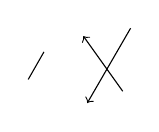
\begin{tikzpicture}\draw(-.5,-.2)--(-.3,.15);\draw[->](.7,-.35)--(.2,.35);\draw[->](.8,.45)--(.25,-.5);\end{tikzpicture}}
\[
\deleted{\unsure{A}}\quad\mathcal F(X^\vee)\ ?
\]
\diagram{\begin{tikzcd}
\mathrm{Top}(A)\arrow[r,"\varphi"]&X\arrow[r,no head,"\psi"]&\mathrm{Top}(B)
\end{tikzcd}}
\diagram{\begin{tikzcd}A\arrow[r]&\unsure{\mathrm{Pt}}(X)\end{tikzcd}}
\[
\deleted{(A\times X)^\wedge\simeq\underline{\mathrm{Hom}}(}
\]
\[
\varphi_*^\vee(F),\quad F\in\mathcal F(\mathrm{Top}(A^\circ))=A^\vee
\]
\[
\psi^*(G),\quad G\in\mathrm{Ob}\,B^\vee
\]
}
\scanpage{10}
\mspage{\textcircled{4}}
% archive foliation: 9
\deleted{$\widehat A\quad A^\vee$}
\[
\boxed{\begin{aligned}
\langle\Phi_*,f^{\circ *}(\Psi^*)\rangle_A&\simeq\langle f_!(\Phi_*),\Psi^*\rangle_B\\
\langle f^*(\Psi_*),\Phi^*\rangle_A&\simeq\langle\Psi_*,f^\circ_!(\Phi^*)\rangle
\end{aligned}}
\]
\margin{\deleted{\unsure{si} $f^{\unsure{\circ}}$ \unsure{iso}}}
\scanpage{11}
\mspage{\textcircled{5}}
% archive foliation: 10
\deleted{$\unsure{HC|H^C}$}
\diagram{\begin{tikzcd}A\arrow[r,hook,"\text{pl fid}"']&B\end{tikzcd}}
\[
x\in B\qquad H_x\in\widehat A\qquad H_x(a)=\mathrm{Hom}_B(a,x)
\]
\[
H^x\in A^\vee\qquad H^x(\cdot)=\mathrm{Hom}_B(a,x)
\]
\[
H_x(a)\times H^x(b)\xrightarrow{\alpha_x}\mathrm{Hom}_A(a,b)
\]
Soit $\unsure{\widetilde{\widetilde A}|\widetilde A}_{\deleted{\unsure{*}}}$ la catégorie des triples $(H_*,H^*,\alpha)$
\unsure{i.e.}
\[
H_*\in\widehat A,\quad H^*\in A^\vee,\quad
\alpha:H_*(a)\times H^*(b)\longrightarrow\mathrm{Hom}_A(a,b)
\]
(bifonctoriel)

les flèches
\[
(H_*,H^*,\alpha)\xrightarrow{\varphi}(H'_*,H'^*,\alpha')
\]
étant données par
\[
\left\{\begin{aligned}
\varphi_*:H_*&\longrightarrow H'_*&&\text{dans }\widehat A\\
\varphi^*:H'^*&\longrightarrow H^*&&\text{dans }A^\vee
\end{aligned}\right.
\]
tels que \deleted{\unsure{l'}} l'on ait
\margin{\diagram{\begin{tikzcd}[row sep=small,column sep=small]
a\arrow[d,"u"']\arrow[dr,"(u')"]&\\
x\arrow[r]\arrow[d,"(v)"']&x'\arrow[dl,"v'"]\\
b&
\end{tikzcd}}}
\diagram{\begin{tikzcd}[row sep=large,column sep=small]
\unsure{u\in}\ \deleted{\unsure{a}}H_*(a)\arrow[d,"\varphi_*"']&\times&H^*(b)\arrow[rr,no head,"\alpha_{a,b}"]&&\mathrm{Hom}(a,b)\arrow[d,equal]\\
H'_*(a)&\times&H'^*(b)\arrow[u,"\varphi'_*"']\arrow[rr,no head,"\alpha'_{a,b}"']&&\mathrm{Hom}(a,b)\\
&&\unsure{v'}\arrow[u,phantom,"\in" description]&&
\end{tikzcd}}
\[
\alpha_{a,b}(u,\varphi'_*(\unsure{v'|u'}))=\alpha'_{a,b}(\varphi_*(u),\unsure{v'|u'})
\]
\deleted{Soit $\unsure{A^\sim}$}
Pour un foncteur pl. fid \(A\xrightarrow{\varphi}B\), on déduit un foncteur
\[
\begin{aligned}
\varphi^{\unsure{\sharp|\natural}}:B&\longrightarrow\widetilde A\\
x&\longmapsto(\varphi^*_{\unsure{(!)}}(\unsure{a|x}),\varphi^{\circ *}(\unsure{a|x}),\alpha_x)
\end{aligned}
\]

\margin{\figure{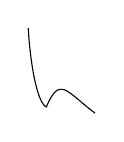
\begin{tikzpicture}\draw(0,1)..controls(.03,.5)and(.12,.05)..(.23,0)..controls(.4,.4)and(.48,.2)..(.85,-.08);\end{tikzpicture}}}
\scanpage{12}
\mspage{\textcircled{6}}
% archive foliation: 11
\uline{NB} $\widetilde{A^\circ}\simeq\widetilde A^\circ$ canonique

$\varphi^{\circ\unsure{\sharp|\natural}}$ s'identifie à $(\varphi^{\unsure{\sharp|\natural}})^\circ$

\figure{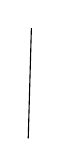
\begin{tikzpicture}\draw(0,0)--(.04,1.4);\end{tikzpicture}}
\margin{Cas où $\varphi^{\unsure{\sharp|\natural}}$ est pl. fidèle ?
Il suffit que $f$ soit strict. génér. ou fon. cogénérateur.}

Cas \diagram{\begin{tikzcd}A\arrow[r,"\varphi=h_A"]&\widehat A\end{tikzcd}}
\deleted{$\unsure{F}$}
\[
\varphi^{\unsure{\sharp|\natural}}_{\deleted{\unsure{a}}}(F)_*=F
\qquad
\underbrace{\varphi^{\unsure{\sharp|\natural}}(F)^*}_{F^{\unsure{\sharp|\natural}}}(a)=\mathrm{Hom}(F,a)
\]
\margin{\figure{\begin{tikzpicture}\draw(0,0)--(.3,1.4);\end{tikzpicture}}$\varphi^{\unsure{\sharp|\natural}}$ fidèle}
\diagram{\begin{tikzcd}[column sep=large]
F\arrow[d,"\varphi_*"']&F^{\unsure{\sharp|\natural}}\\
\unsure{F'|G}&\unsure{F'|G}^{\unsure{\sharp|\natural}}\arrow[u,"\varphi^*"']
\end{tikzcd}}
\inserted{$(\stackrel{?}{=}\varphi_*^{\unsure{\sharp|\natural}})$}
\figure{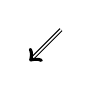
\begin{tikzpicture}\draw[->,double](.4,.4)--(0,0);\end{tikzpicture}}
tels que $u\in F(a)$, $u'\in\unsure{F'|G}^{\unsure{\sharp|\natural}}(b)$ implique
(i.e. $a\longrightarrow F\quad\unsure{F'|G}\longrightarrow b$)
\figure{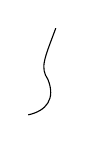
\begin{tikzpicture}\draw(0,1.1)..controls(-.15,.7)and(-.2,.6)..(-.1,.45)..controls(0,.2)and(-.12,.05)..(-.35,0);\end{tikzpicture}}
\margin{\deleted{$\unsure{\varphi}$}\diagram{\begin{tikzcd}A\arrow[r,bend right]&e\arrow[l,bend right]\end{tikzcd}}}
\diagram{\begin{tikzcd}[column sep=large,row sep=large]
a\arrow[dr,"u"']\arrow[drr,bend left=18,"u'=\varphi_*(u)\deleted{\unsure{\varphi^*}}=\varphi\circ u"]&&\\
&F\arrow[r,"\varphi_*"]\arrow[dl,"v"']&G\arrow[dll,bend left=15,"v'"']\\
b&&
\end{tikzcd}}
\margin{\deleted{$\unsure{v'\varphi_*}$}\figure{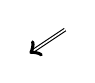
\begin{tikzpicture}\draw[->,double](.45,.3)--(0,0);\end{tikzpicture}}}
\margin{comm.\quad comm ?}
\[
v=v'\circ\varphi_*\ ?
\]
On sait que $v\circ u=v'\circ u'=v'(\unsure{\varphi|\varphi_*}u)=(v'\varphi_*)u$

\uline{Considérons} alors la \deleted{image essentielle} sous catégorie pleine de
$\unsure{\widetilde{\widetilde A}|\widetilde A}$
\deleted{\unsure{réciproquement}}
\deleted{formée des}
\inserted{dont l'un des objets est}
\unsure{la réunion} des \unsure{images} essentielles de
\[
F\qquad G
\]
\figure{\begin{tikzpicture}\draw(0,0)--(0,.2);\end{tikzpicture}}
\diagram{\begin{tikzcd}
\Psi_1^\circ\arrow[r,no head]&a\arrow[r]&\Phi\arrow[r]&\Psi_2^\circ
\end{tikzcd}}
\diagram{\begin{tikzcd}[row sep=small,column sep=small]
\Phi_1\arrow[r]\arrow[d,equal]&\Psi\arrow[rr,no head]\arrow[d,equal]\arrow[dr]&&\Phi_2\\
\underset{i}{\lim}\,a_i&\cdot&a\arrow[ur]&
\end{tikzcd}}
\figure{\begin{tikzpicture}\draw(0,0)..controls(2,-.1)and(3,-.1)..(3.5,.3)..controls(4,1)and(4.5,2.6)..(5.3,3.3)..controls(5.8,3.8)and(7,3.7)..(8,3.8);\end{tikzpicture}}
\[
\widetilde A\subset
\]
\diagram{\begin{tikzcd}[row sep=small,column sep=large]
F,&G\\
\widehat A\arrow[u]&A^\vee\arrow[u]
\end{tikzcd}}
ou bien \deleted{$\unsure{G=}$}
\[
(F,G,\alpha)\simeq(F,F^{\unsure{\sharp|\natural}},\alpha_F)
\]
\[
(F,G,\alpha)\simeq(G^{\unsure{b|\flat}},G,\alpha^G)
\]
\diagram{\begin{tikzcd}a\arrow[r]&F\arrow[l,bend left=25]\end{tikzcd}}
\diagram{\begin{tikzcd}[row sep=large,column sep=large]
A\arrow[d,"f"']&\widetilde A&\widehat A\\
B&\widetilde B\arrow[u,"\widetilde f"']&\widehat B\arrow[u,"f^*"']
\end{tikzcd}}
\figure{\begin{tikzpicture}\draw(0,0)--(.8,2);\end{tikzpicture}}
\diagram{\begin{tikzcd}[row sep=large,column sep=large]
\widehat A\arrow[d,"f_!"']&A\arrow[d,"f"']&A^\vee\arrow[d,"f^\circ_!"]&A^\vee\\
\widehat B&B&B^\vee&B^\vee\arrow[u,"f^{\circ *}"]
\end{tikzcd}}
\diagram{\begin{tikzpicture}
\node at (0,0){\begin{tikzcd}[row sep=large,column sep=large]
\widehat A\arrow[r,hook]&\widetilde A\arrow[d,"\widetilde f"]&A^{\vee\circ}\arrow[l,hook']\\
\widehat B\arrow[u,"f^*"']\arrow[r,hook]&\widetilde B&B^{\vee\circ}\arrow[l,hook']\arrow[u,"f^{\circ *\circ}"]
\end{tikzcd}};
\draw(0,0) ellipse(4.4cm and 2.3cm);
\end{tikzpicture}}
\scanpage{13}
% archive foliation: 12

\texttt{STMT NO. MESSAGE}

\texttt{4 IEF653I SUBSTITUTION JCL - PGM=CRBATCH,REGION=100K,PARM=}

\texttt{\$HASP373 STARTED - INIT 10 - CLASS Q - SYS E333}

\texttt{IEF236I ALLOC. FOR PREDONTA CSSBATCH}

\texttt{IEF237I 381 ALLOCATED TO STEPLIB}

\texttt{IEF237I 2C9 ALLOCATED TO SYS00206}

\texttt{IEF237I VIO ALLOCATED TO SYSUT1}

\texttt{IEF237I JES2 ALLOCATED TO SYSPRINT}

\texttt{IEF237I SHR ALLOCATED TO CRJIF}

\texttt{IEF237I JES2 ALLOCATED TO SYSTA}

\texttt{IEF237I 59F ALLOCATED TO SYS00002}

\texttt{IEF237I 59F ALLOCATED TO SYS00001}

\texttt{IEF285I CRAY1.PREDONTA.CS.D82153.T111736.R43 CATALOGED}

\texttt{IEF285I VOL SER NOS= CRAY11.}

\texttt{CSS2060 - JOB QUEUED FOR TRANSFER}

\texttt{IEF142I PREDONTA CSSBATCH - STEP WAS EXECUTED - COND CODE 0000}

\texttt{IEF285I CIS1.PROD.CSSBATCH.V1.\unsure{AY81} KEPT}

\texttt{IEF285I VOL SER NOS= MVS104.}

\texttt{IEF285I SYSCTLG.VSAC015 KEPT}

\texttt{IEF285I VOL SER NOS= SAC015.}

\texttt{IEF285I SYS82153.\unsure{T111736}.RA008.PREDONTA.SYSUT1 DELETED}

\texttt{IEF285I JES2.JOB00653.S000102 SYSOUT}

\texttt{IEF285I SYS1.CR.JIF KEPT}

\texttt{IEF285I VOL SER NOS= CRAY11.}

\texttt{IEF285I JES2.JOB00653.\unsure{ST0101|SI0101} SYSIN}

\texttt{IEF285I SYSCTLG.VCRAY11 KEPT}

\texttt{IEF285I VOL SER NOS= CRAY11.}

\texttt{IEF373I STEP /CSSBATCH/ START 82153.1117}

\texttt{IEF374I STEP /CSSBATCH/ STOP 82153.1117 CPU 0MIN 00.20SEC SRB 0MIN 00.02SEC VIRT 84K SYS 248K}

\texttt{IEF375I JOB /PREDONTA/ START 82153.1117}

\texttt{IEF376I JOB /PREDONTA/ STOP 82153.1117 CPU 0MIN 00.20SEC SRB 0MIN 00.02SEC}
\scanpage{14}
\mspage{7}
% archive foliation: 13

\diagram{
\begin{tikzcd}[column sep=large,row sep=large]
&& \underline{\mathrm{Hom}}(A^\vee,\unsure{(Ens)}) \\
\widehat A \arrow[r,"\approx"] & \underline{\mathrm{Hom}}_!(A^\vee,Ens) \arrow[ur,hook] && A^{\vee\circ} \arrow[ul,hook] \arrow[r,"\approx"] & \underline{\mathrm{Hom}}_{rep}(A^\vee,(Ens)) \\
&& (Kar(A^\circ))^\circ \simeq Kar(A) \arrow[ul,hook] \arrow[ur,hook] \\
&& \unsure{\overline A|\widetilde A} \arrow[u,hook] \\
&& A \arrow[u,hook]
\end{tikzcd}}

\[\overline{\widetilde{\unsure{\mathcal E|E}}}(A)\]

\diagram{
\begin{tikzcd}[row sep=large,column sep=large]
& \underline{\mathrm{Hom}}(A^{\unsure{\vee|\circ}},(Ens)) & \\
& \mathcal E(A) \arrow[u,hook,"\mathrm{pl.\ fid.}"] & \\
\widehat A \arrow[ur,hook] && A^{\vee\circ} \arrow[ul,hook] \\
& A=\widehat A\unsure{\cap|,}A^{\vee\circ} \arrow[ul,hook] \arrow[ur,hook] &
\end{tikzcd}}

\figure{\begin{tikzpicture}
\draw (0,3.8) .. controls (2.3,4.5) and (3.6,4.4) .. (4.7,3.5) .. controls (7,1.4) and (9,0.1) .. (10,0);
\end{tikzpicture}}

\diagram{
\begin{tikzcd}[row sep=large,column sep=large]
& M & \\
M_1 \arrow[ur,hook] && M_2 \arrow[ul,hook] \\
& \deleted{\unsure{M_\epsilon}}\inserted{\unsure{N}} \arrow[ul,hook] \arrow[ur,hook] & \\
M'_1 \arrow[uu,hook,"\deleted{\unsure{\mathrm{pl.\ fid.}}}"] && M'_2 \arrow[uu,hook,"\deleted{\unsure{\mathrm{pl.\ fid.}}}"'] \\
& N' \arrow[ul,hook] \arrow[ur,hook] \arrow[uu,hook,"\deleted{\unsure{M_0}}\;\deleted{\unsure{\mathrm{pl.\ fid.}}}"] &
\end{tikzcd}}

\[N=M_1\cap M_2\]
\unsure{Ttes} les flèches pl. fid.

Alors on définit une catégorie $\Sigma'$, somme des sous-catégories pleines $M'_1$ et $M'_2$, avec \unsure{int.} $N'$, et un foncteur pl. fid. $\Sigma'\to M$ (factorisant par $M_1\cup M_2$). Mais $=$ si $M_1,M_2$ \uline{\unsure{ss.}} pleines en $M$ (avec $N$ donc pl. en $M$), et $M'_1-M_1$, $M'_2-M_2$ des équiv., $M'_1$ et $M'_2$ ne sont pas \unsure{néct.} \unsure{ss.} pl. \unsure{ds.|de} $\Sigma'$, et $N'-N$ n'est pas tjrs une équivalence.
\scanpage{15}
% archive foliation: 14

\[
\underline{\mathrm{Hom}}(A,M)\simeq
\underline{\mathrm{Hom}}_!(\widehat A,M)\simeq
\mathrm{Hom}_!(\widehat A_{ab},M).
\]
\[\deleted{\unsure{\sharp}}\]
\figure{\begin{tikzpicture}\draw (0,0) -- (.20,.02) -- (.36,-.04);\draw (.55,.15)--(.9,.15);\end{tikzpicture}}

\uline{Ex} $M=\unsure{Ab}$
\diagram{\begin{array}{c}
\underline{\mathrm{Hom}}(B^\circ,\unsure{Ab|M_b})\simeq\widehat B_{ab}\\
\rotatebox{90}{$\simeq$}\\
\mathrm{Hom}_!(\widehat A_{ab}
\end{array}}

\figure{\begin{tikzpicture}\draw (0,0)--(.01,.13);\fill (.02,.19) circle (.012);\end{tikzpicture}}

\[A=B^\circ\quad|\quad B=A^\circ\]

\diagram{\begin{array}{lll}
\underline{\mathrm{Hom}}_{\deleted{\unsure{\sharp}}}(A,M)\simeq
\mathrm{Hom}^{\deleted{\unsure{\sharp}}}_!(\widehat A,M)
& \deleted{\unsure{\text{cofaisceaux}}} & \text{cofaisceaux sur }A,\ \text{à val. dans }M.\\
\rotatebox{90}{$\simeq$} &&\\
\underline{\mathrm{Hom}}(B^\circ,M)\simeq\mathrm{Hom}^!(\widehat B^\circ,M)
&&\text{faisceaux sur }B,\ \text{à val. dans }M.
\end{array}}

\diagram{\begin{array}{c}
\mathcal F(\mathcal X,M)^\circ\simeq\mathcal F^\vee(\mathcal X,M^\circ)\\
\rotatebox{90}{$\equiv$}\\
(\mathrm{Hom}^!(A,M))^\circ\\
\rotatebox{90}{$\simeq$}\\
\mathrm{Hom}_!(A^\circ,M^\circ)
\end{array}}

$\mathcal F(\mathcal X,M)$ et $\mathcal F^\vee(\mathcal X,M^\circ)$ sont \unsure{duals|duales} l'une de l'autre
\[
\mathcal F(\mathcal X,M)\simeq\mathcal F^\vee(\mathcal X^\circ,M)
\]
\[
\underline{\mathrm{Hom}}^!(A^\circ,M)\simeq\underline{\mathrm{Hom}}_!(A,M^\circ)^\circ
\]
